\begin{appendices}

%Some Table of Contents entry formatting
\addtocontents{toc}{\protect\renewcommand{\protect\cftchappresnum}{\appendixname\space}}
\addtocontents{toc}{\protect\renewcommand{\protect\cftchapnumwidth}{6em}}

%Begin individual appendices, separated as chapters

\chapter{Notation}\label{appendix:0}

\section*{Array Notation for Tensors}

We outline the array notation used on relevant tensor quantities for the 
computer implementation of the work presented in the chapters of this 
manuscript. The relevant cases are i) the three dimensional state and ii) the 
plane stress state. For each one, we show how second order stress and strain 
tensors, on one hand, and fourth order material constitutive tensor on the 
other, are stored in computer memory as one dimensional and two dimensional 
arrays (``vectors").

\subsection*{Three Dimensions}

For the symmetric second order stress tensor $\bm{\sigma}$ we have:
\begin{equation*}
	\boldsymbol{\sigma} = \begin{bmatrix}
		\sigma_{11} & \sigma_{12} & \sigma_{13} \\
		\sigma_{12} & \sigma_{22} & \sigma_{23} \\
		\sigma_{13} & \sigma_{23} & \sigma_{33} \\
	\end{bmatrix}\rightarrow \bvec{\sigma} = \begin{bmatrix}
		\sigma_{11} & \sigma_{22} & \sigma_{33} & \sigma_{12} & \sigma_{23} & 
		\sigma_{13}
	\end{bmatrix}^T
\end{equation*}

\noindent Similarly, for the symmetric second order strain tensor we have:
\begin{equation*}
	\boldsymbol{\epsilon} = \begin{bmatrix}
		\epsilon_{11} & \epsilon_{12} & \epsilon_{13} \\
		\epsilon_{12} & \epsilon_{22} & \epsilon_{23} \\
		\epsilon_{13} & \epsilon_{23} & \epsilon_{33} \\
	\end{bmatrix}\rightarrow \bvec{\epsilon} = \begin{bmatrix}
		\epsilon_{11} & \epsilon_{22} & \epsilon_{33} & 2\epsilon_{12} & 
		2\epsilon_{23} & 
		2\epsilon_{13}
	\end{bmatrix}^T
\end{equation*}
and it is assumed that for the engineering strains we have 
$\gamma_{ij}=2\epsilon_{ij}$, $i\neq j$.

The stress and strain convention is extended to all other second order 
symmetric tensors involved in the formulation of the stress update algorithm, 
such as back-stress or effective stress tensors or the plastic strain tensor.

The fourth order elastic constitutive tensor, $\mathbb{C}$, is represented as a 
two dimensional matrix $\bmat{C}$ as follows:
\begin{equation*}
	\bmat{C} = \begin{bmatrix}
		C_{1111} & C_{1122} & C_{1133} & C_{1112} & C_{1123} & C_{1113}\\
		C_{2211} & C_{2222} & C_{2233} & C_{2212} & C_{2223} & C_{2213}\\
		C_{3311} & C_{3322} & C_{3333} & C_{3312} & C_{3323} & C_{3313}\\
		C_{1211} & C_{1222} & C_{1233} & C_{1212} & C_{1223} & C_{1213}\\
		C_{2311} & C_{2322} & C_{2333} & C_{2312} & C_{2323} & C_{2313}\\
		C_{1311} & C_{1322} & C_{1333} & C_{1312} & C_{1323} & C_{1313}
	\end{bmatrix}
\end{equation*}

so that:
\begin{equation*}
	\text{ARRAY}(d\bm{\sigma})=\text{ARRAY}(\mathbb{C}:d\bm{\epsilon})=
	\bmat{C}d\bvec{\epsilon} =d\bvec{\sigma}
\end{equation*}

For problems in elasticity and associative plasticity, the material 
constitutive tensor possesses minor and major symmetries:
$$\mathbb{C}_{ijkl}=\mathbb{C}_{jikl}=\mathbb{C}_{jilk}=\mathbb{C}_{klij}$$

For isotropic linear elasticity, $\bmat{C}$ is given as follows:
\begin{equation*}
	\bmat{C} = \frac{E}{(1+\nu)(1-2\nu)}\begin{bmatrix}
		1-\nu & \nu & \nu & 0 & 0 & 0\\
		\nu & 1-\nu & \nu & 0 & 0 & 0\\
		\nu & \nu & 1-\nu & 0 & 0 & 0\\
		0 & 0 & 0 & \frac{1-2\nu}{2} & 0 & 0\\
		0 & 0 & 0 & 0 & \frac{1-2\nu}{2}  & 0\\
		0 & 0 & 0 & 0 & 0 & \frac{1-2\nu}{2} \\
	\end{bmatrix}
\end{equation*}

Enforcement of the zero-stress condition $\sigma_{22}=\sigma_{33}$ at a fiber, 
after the plastic parameter is determined, requires a local iterative procedure 
whereby $\bmat{C}$ is decomposed in accordance to the active and zero stress 
components. The local iteration formula for the three dimensional algorithm 
takes the following form:

\begin{equation*}
	\begin{bmatrix}
		\Delta \epsilon_{22}\\
		\Delta \epsilon_{33}
	\end{bmatrix} = -\begin{bmatrix}
	C_{2222} & C_{2233}\\
	C_{3322} & C_{3333}
\end{bmatrix}^{-1}\begin{bmatrix}
\sigma_{22}\\
\sigma_{33}
\end{bmatrix}
\end{equation*}
\noindent where for each corrected increment in $\Delta\epsilon_{22}$, 
$\Delta\epsilon_{33}$, the stress update has to be repeaded until 
max($\vert\sigma_{22}\vert$,$\vert\sigma_{33}\vert$)$\leq \epsilon_{tol}$, with 
$\epsilon_{tol}$ being a user-specified tolerance. When convergence has been 
achieved, only then state variables for a fiber are updated.

Note that the same convention is used for the continuous or the consistent 
tangent moduli.

\subsection*{Plane Stress}

Here, the vectorization of stress and strain tensors is implemented as follows:
\begin{equation*}
	\bm{\sigma}=\begin{bmatrix}
		\sigma_{11} & \sigma_{12}\\
		\sigma_{12} & \sigma_{22}
	\end{bmatrix}\rightarrow \bvec{\sigma}=\begin{bmatrix}
	\sigma_{11}\\ \sigma_{22} \\ \sigma_{12}
\end{bmatrix},\quad 
	\bm{\epsilon}=\begin{bmatrix}
	\epsilon_{11} & \epsilon_{12}\\
	\epsilon_{12} & \epsilon_{22}
\end{bmatrix}\rightarrow \bvec{\epsilon}=\begin{bmatrix}
	\epsilon_{11}\\ \epsilon_{22} \\ 2\epsilon_{12}
\end{bmatrix}
\end{equation*}

The matrix representation of $\mathbb{C}$ associated with the plane-stress 
condition is:
\begin{equation*}
	\bmat{C}=\begin{bmatrix}
		C_{1111} & C_{1122} & C_{1112}\\
		C_{2211} & C_{2222} & C_{2212}\\
		C_{1211} & C_{1222} & C_{1212}
	\end{bmatrix}
\end{equation*}

For isotropic linear elasticity in plane stress conditions, we have for 
$\bmat{C}$:

\begin{equation}
	\bmat{C} = \frac{E}{1-\nu^2}\begin{bmatrix}
		1 & \nu & 0\\
		\nu & 1 & 0\\
		0 & 0 & \frac{1-\nu}{2}
	\end{bmatrix}
\end{equation}

The local Newton iteration to enforce condition $\sigma_{22}=0$ during the 
fiber stress update, typically required when the plane-stress return mapping 
algorithm by Simo\cite{Simo1} is used, takes the following form:
\begin{equation*}
	\Delta\epsilon_{22} = -\frac{1}{C_{2222}}\sigma_{22}
\end{equation*}


\section*{Analysis Operators}

We adopt the notation $\bvec{F}:\mathbb{R}^n\rightarrow\mathbb{R}^m$ to 
indicate a 
mapping $\bvec{F}$ that takes as argument a vector of dimension $n$, 
$\bvec{x}\in\mathbb{R}^n$, and maps it onto a vector of dimension $m$, 
$\bvec{y}\in\mathbb{R}^m$:
\begin{equation*}
	\bvec{y} = \bvec{F}(\bvec{x})
\end{equation*}

We note that operations involving the symbol $\nabla$ map scalars to
vectors and vectors to matrices. For example, if $f:\mathbb{R}^p\rightarrow 
\mathbb{R}$ and
$\bvec{v}:\mathbb{R}^p\rightarrow\mathbb{R}^q$, then $\nabla
f:\mathbb{R}^p\rightarrow\mathbb{R}^p$ and
$\nabla\bvec{v}:\mathbb{R}^p\rightarrow\mathbb{R}^{p\times q}$. For a scalar 
function 
$f(\bvec{x})$, $\bvec{x}\in\mathbb{R}^n$ we have:
\begin{equation*}
	\nabla f = \begin{bmatrix}
		\displaystyle\frac{\partial f}{\partial x_1} & \dots & 
		\displaystyle\frac{\partial f}{\partial x_n}
	\end{bmatrix}^T
\end{equation*}

\subsection*{Jacobian of Smooth Maps}
The Jacobian of $\bvec{F}$, denoted $\bmat{J}$, is an $m\times n$ matrix 
expressed as 
follows:
\begin{equation*}
	\bmat{J} = \begin{bmatrix}
		\nabla_{\bm{x}}F_1^T\\
		\vdots\\
		\nabla_{\bm{x}}F_m^T\\
	\end{bmatrix} = \begin{bmatrix}
		\displaystyle	\frac{\partial \bvec{F}}{\partial x_1} & \dots & 
		\displaystyle\frac{\partial \bvec{F}}{\partial 
			x_n}\end{bmatrix} = \begin{bmatrix}
		\displaystyle\frac{\partial F_1}{\partial x_1} & \dots & 
		\displaystyle\frac{\partial F_1}{\partial x_n}\\
		\vdots & \ddots & \vdots\\
		\displaystyle\frac{\partial F_m}{\partial x_1} & \dots & 
		\displaystyle\frac{\partial F_m}{\partial x_n} 
	\end{bmatrix}
\end{equation*}

\chapter{Gradient of Hybrid NLP Lagrangian}\label{appendix:A}

Explicit expressions of the beam formulation are provided in this
Appendix. 

The Lagrangian function is used here, as presented in Eq.
(\ref{eq:langrT}):
\begin{gather}
	\mathcal{L}(\bvec{y}, \bvec{d}_g,\bvec{\lambda}) =
	U-W+\bvec{\lambda}^T\bvec{h}_g
	\label{eq:globalL}
\end{gather}

\noindent where it is also reminded that $\bvec{y} = \begin{bmatrix}
	\bvec{y}_1^T & \bvec{y}_2^T & \cdots & \bvec{y}_m^T
\end{bmatrix}^T$, $\bvec{y}_i = \begin{bmatrix}
	\bvec{q}_i & \phi_i
\end{bmatrix}^T$ and $\bvec{q}_i = \begin{bmatrix}
	\epsilon_i & \gamma_i & \kappa_i
\end{bmatrix}^T$. The number $m$ designates the \emph{total} number of
integration points in the structure.

%\subsection{Gradient of Strain Energy}
The gradient of the strain energy, $U$, is expressed as:
\begin{gather}
	\nabla U = \begin{bmatrix}
		\nabla_{\mathbf{y}}U\\ \nabla_{\mathbf{d}_g}U\\ 
		\nabla_{\mathbf{\lambda}}U
	\end{bmatrix}\nonumber
\end{gather}

\noindent The gradient with respect to the strain vector $\bvec{y}$ gives the
stress resultants at all cross-sections and has the following form for a
particular cross-section $i$:
\begin{gather}
	\nabla_{\mathbf{y}_i}U = \begin{bmatrix}
		w_iN_i\\ w_iV_i\\ w_iM_i\\ 0
	\end{bmatrix} = w_i\begin{bmatrix}
		\bvec{F}_{sec}^{(i)}\\ 0
	\end{bmatrix}
	\label{eq:straingrad}
\end{gather}

\noindent it is usually computed by numerical integration of Eqs.
(\ref{eq:fsecx}) over the cross-section height. In the case of elastic
analysis, the above vector can be computed explicitly for each cross-section,
since then $\bvec{F}_{sec}^{(i)} = \begin{bmatrix}
	EA\epsilon_i & k_sGA\gamma_i & EI\kappa_i
\end{bmatrix}^T$.

The gradients of $U$ with respect to both $\bvec{d}_g$ and $\bvec{\lambda}$
provide zero vectors:
\begin{gather}
	\nabla_{\mathbf{d}_g}U = 
	\bvec{0}\in\mathbb{R}^{3N_{nod}}\quad\text{and}\quad
	\nabla_{\mathbf{\lambda}}U = \bvec{0}\in\mathbb{R}^{s}\nonumber
\end{gather}

\noindent where $s=m + 3n_{el}$, $n_{el}$ being the number of elements.
Finally, we then get:
\begin{gather}
	\nabla U = \begin{bmatrix}
		\nabla_{\mathbf{y}}U\\ \bvec{0}\\ \bvec{0}
	\end{bmatrix}
\end{gather}

%\subsection{Gradient of Constraints}

We restate the constraints equations from Eqs.
(\ref{eq:impsd1})-(\ref{eq:impsd2}):
\begin{gather}
	\bvec{h}_g = \begin{bmatrix}
		\bvec{h}_g^A\\ \bvec{h}_g^B
	\end{bmatrix} =
	\begin{bmatrix}
		\bmat{V}_1\bvec{d}_g - \bmat{\Lambda}^T\bigg[\sum_{i=1}^n
		w_i\bmat{R}_i(\bvec{q}_i+\bvec{E}_1) - \ell\bvec{E}_1\bigg]\\
		\bvec{\phi}-\bmat{V}_2\bvec{d}_g - \bmat{T}\bvec{\kappa}
	\end{bmatrix}\nonumber
\end{gather}

\noindent For notational simplicity, we assume here only one element
in the derivations that follow. When more elements are used, their
corresponding constraint vectors are stacked in vector form as
$\bvec{h} = \begin{bmatrix}
	\ \bvec{h}_g^{1\ T}& \bvec{h}_g^{2\ T}& \cdots & \bvec{h}_g^{n_{el}\ T}
\end{bmatrix}^T$.
The gradient with respect to the strain vector
$\bvec{y}_i$ at a particular cross-section is given by:
\begin{gather}
	\nabla_{\mathbf{y}_i}\bvec{h}_g^A = \begin{bmatrix}
		\nabla_{\mathbf{q}_i}\bvec{h}_g^A &\ \dfrac{d \bvec{h}_g^A}{d\phi_i}
	\end{bmatrix} = -w_i\bmat{\Lambda}^T\begin{bmatrix}
		\bmat{R}_i &\
		\bmat{R}_i\bmat{X}[\bvec{q}_i+\bvec{E}_1]
	\end{bmatrix}\nonumber
\end{gather}

\noindent where:
\begin{gather}
	\frac{d\bmat{R}_i}{d\phi_i} = \bmat{R}_i\bmat{X}\quad\text{and}\quad
	\bmat{X} = \begin{bmatrix}
		0 & -1 & 0\\
		1 &  0 & 0\\
		0 &  0 & 0
	\end{bmatrix}\nonumber
\end{gather}

\noindent The gradient of $\bvec{h}_g^B$ with respect to strain vector
$\bvec{y}_i$, is:
\begin{gather}
	\nabla_{\mathbf{y}_i}\bvec{h}_g^B = \begin{bmatrix}
		\nabla_{\mathbf{q}_i}\bvec{h}_g^B & \dfrac{d \bvec{h}_g^B}{d\phi_i}
	\end{bmatrix} = \begin{bmatrix}
		\bvec{0} & \bvec{0} & -\bmat{T}\hat{\mathbf{E}}_i & \hat{\mathbf{E}}_i
	\end{bmatrix}
	\label{eq:grad_Hb_y}
\end{gather}

\noindent where $\hat{\mathbf{E}}_i\in\mathbb{R}^{n_q}$ is a unit vector with 
the
$i$-th component equal to one.
\noindent Collectively, we have:
\begin{gather}
	\nabla_{\mathbf{y}_i}\bvec{h}_g = \begin{bmatrix}
		-w_i\bmat{\Lambda}^T\bmat{R}_i & -w_i\bmat{\Lambda}^T
		\bmat{R}_i\bmat{X}[\bvec{q}_i+\bvec{E}_1]\\
		[\bvec{0}\quad \bvec{0}\quad -\bmat{T}\hat{\mathbf{E}}_i] & 
		\hat{\mathbf{E}}_i
	\end{bmatrix}
	\label{eq:con1}
\end{gather}

\noindent The gradient with respect to the displacement vector is derived in a
straightforward manner by simple derivations:
\begin{gather}
	\nabla_{\mathbf{d}_g}\bvec{h}_g = \begin{bmatrix}
		\bmat{V}_1 \\ -\bmat{V}_2
	\end{bmatrix}
	\label{eq:congradisp}
\end{gather}

\begin{gather}
	\bmat{V}_1 = \begin{bmatrix}
		-\bmat{I} & \bmat{I}
	\end{bmatrix}\quad\text{,}\quad
	\bmat{V}_2 = \begin{bmatrix}
		\bvec{0} & \bvec{0} & \bvec{1} & \bvec{0} & \bvec{0} & \bvec{0}
	\end{bmatrix}\nonumber\\
	\bmat{I} = \begin{bmatrix}
		1 & 0 & 0\\
		0 & 1 & 0\\
		0 & 0 & 1
	\end{bmatrix}\quad\text{,}\quad \bvec{0},\bvec{1}\in\mathbb{R}^{n_q},\quad 
	\bvec{0}=\begin{bmatrix}
		0 & \cdots & 0
	\end{bmatrix}^T,\quad \bvec{1}=\begin{bmatrix}
		1 & \cdots & 1
	\end{bmatrix}^T\nonumber
\end{gather}

\noindent Finally, the gradient with respect to the vector $\bvec{\lambda}$
gives a zero matrix:
\begin{gather}
	\nabla_{\mathbf{\lambda}}\bvec{h}_g = 
	\bmat{0}\in\mathbb{R}^{(n_q+3)\times(n_q+3)}
\end{gather}

\noindent The total constraints gradient is then expressed in block matrix
form as:
\begin{gather}
	\nabla\bvec{h}_g = \begin{bmatrix}
		\nabla_{\mathbf{y}_1}\bvec{h}_g & \nabla_{\mathbf{y}_2}\bvec{h}_g &
		\cdots & \nabla_{\mathbf{y}_{n_q}}\bvec{h}_g & 
		\nabla_{\mathbf{d}_g}\bvec{h}_g &
		\nabla_{\mathbf{\lambda}}\bvec{h}_g
	\end{bmatrix}\nonumber
\end{gather}

\noindent Note that in the case of small displacements, only the
expression $\nabla_{\mathbf{y}_i}\bvec{h}_g^A$ has to be modified, so that
the strain-displacement relations reduce to the classical linear Timoshenko
theory:
\begin{gather}
	\nabla_{\mathbf{y}_i}\bvec{h}_g^A =-w_i\bmat{\Lambda}^T\begin{bmatrix}
		1 & -\phi_i & 0 & -\gamma_i\\
		0 & 1 & 0 & 1\\
		0 & 0 & 1 & 0
	\end{bmatrix}\nonumber
\end{gather}

\noindent with the vector of constraints $\bvec{h}_g^A$ being:
\begin{gather}
	\bvec{h}^A_g = \bmat{V}_1\bvec{d}_g - \bmat{\Lambda}^T\bigg[\sum_{i=1}^n
	w_i[\hat{\bmat{R}}_i(\bvec{q}_i+\bvec{E}_1) -\bvec{g}_i] - 
	\ell\bvec{E}_1\bigg]
\end{gather}

\noindent where:
\begin{gather}
	\hat{\bmat{R}}_i = \begin{bmatrix}
		1 & -\phi_i & 0\\
		\phi_i & 1 & 0\\
		0 & 0 & 1
	\end{bmatrix},\quad \bvec{g}_i = \begin{bmatrix}
		0\\ \epsilon_i\phi_i\\ 0
	\end{bmatrix}\nonumber
\end{gather}
\noindent The vector $\bvec{g}_i$ is added in order to eliminate the second
order term $\epsilon_i\phi_i$ arising from the imposition of the small
displacement assumption $\sin\phi_i \approx \phi_i$, $\cos\phi_i\approx1$ in Eq.
(\ref{eq:impsd1}).
%\subsection{Gradient of the Potential Energy}

The potential energy due to external loads $\bvec{P}$ is:
\begin{gather}
	W = \sum_{j=1}^{N_{nod}}\bvec{P}_j^T\bvec{d}_{g,j} = 
	\bvec{d}_g^T\bvec{P}\nonumber
\end{gather}

\noindent The gradient of the potential energy is, again, straightforward in its
derivation as it only depends on the displacement vector:
\begin{gather}
	\nabla W = \begin{bmatrix}
		\nabla_{\mathbf{y}}W\\ \nabla_{\mathbf{d}_g}W\\ 
		\nabla_{\mathbf{\lambda}}W
	\end{bmatrix}\nonumber
\end{gather}

\noindent with $\nabla_{\mathbf{y}}W = \bvec{0}\in\mathbb{R}^m$,
$\nabla_{\mathbf{d}_g}W = \bvec{P}$ and $\nabla_{\mathbf{\lambda}}W =
\bvec{0}\in\mathbb{R}^{n_q+3}$ for one element. Thus, we have:
\begin{gather}
	\nabla W = \begin{bmatrix}
		\bvec{0}\\ \bvec{P}\\ \bvec{0}	\end{bmatrix}
\end{gather}

%\subsection{Gradient of the Lagrangian}

Finally, the gradients of the Lagrangian with respect to the three constituent 
vector arguments, $\bvec{y}_i$, $\bvec{d}_g$ and $\bvec{\bm{\lambda}}$ are 
shown below. These expressions are substituted in Eqs. (\ref{eq:eqtot}):

\begin{gather}
	\nabla_{\mathbf{y}_i}\mathcal{L} = w_i\begin{bmatrix}
		\bvec{F}_{sec}^{(i)} \\ 0
	\end{bmatrix} + \begin{bmatrix}
		-w_i\bmat{\Lambda}^T\bmat{R}_i & -w_i\bmat{\Lambda}^T
		\bmat{R}_i\bmat{X}[\bvec{q}_i+\bvec{E}_1]\\
		[\bvec{0}\quad \bvec{0}\quad -\bmat{T}\hat{\mathbf{E}}_i] & 
		\hat{\mathbf{E}}_i
	\end{bmatrix}^T\bvec{\lambda}
	\label{eq:A7}
\end{gather}
\begin{gather}
	\nabla_{\mathbf{d}_g}\mathcal{L} = -\begin{bmatrix}
		\bvec{0}\\ \bvec{P}\\ \bvec{0}	\end{bmatrix} + \begin{bmatrix}
		\bmat{V}_1 \\ -\bmat{V}_2
	\end{bmatrix}^T\bvec{\lambda}
\end{gather}
\begin{gather}
	\nabla_{\bm{\lambda}}\mathcal{L} = \bvec{h}_g
\end{gather}

\chapter{Hessian of Hybrid NLP Lagrangian}\label{appendix:B}
The Hessian form in Eq. (\ref{eq:hess}), is restated here:
\begin{gather}
	\bmat{H} = 	\begin{bmatrix}
		\nabla^2_{\mathbf{yy}}\mathcal{L} & \bmat{0} & 
		\nabla_{\mathbf{y}}\bvec{h}^T_g\\
		\bmat{0} & \bmat{0} & \nabla_{\mathbf{d_g}}\bvec{h}^T_g\\
		\nabla_{\mathbf{y}}\bvec{h}_g & \nabla_{\mathbf{d_g}}\bvec{h}_g & 
		\bmat{0}\\
	\end{bmatrix}\nonumber
\end{gather}

\noindent The gradients of $\bvec{h}_g$ have been derived in the previous
section.  Thus, for the complete specification of the second order information
we need only to determine the second derivative matrix with respect to the
strain vector $\bvec{y}$. Since different integration points are independent of
one another, then it is clear
that $\nabla^2_{\mathbf{y}_i\mathbf{y}_j}\mathcal{L}=\bmat{0}$ for $i\neq j$.
Therefore, the matrix $\nabla^2_{\mathbf{yy}}\mathcal{L}$ has a block diagonal
form:
\begin{gather}
	\nabla^2_{\mathbf{yy}}\mathcal{L} = \begin{bmatrix}
		\nabla^2_{\mathbf{y}_i\mathbf{y}_i}\mathcal{L} &\bmat{0} &\cdots & 
		\bmat{0} \\
		\bmat{0} & \nabla^2_{\mathbf{y}_i\mathbf{y}_i}\mathcal{L} &\cdots 
		&\bmat{0} \\
		\vdots & \ddots & &\vdots \\
		\bmat{0} & \cdots &\bmat{0} & 
		\nabla^2_{\mathbf{y}_m\mathbf{y}_m}\mathcal{L}
	\end{bmatrix}\nonumber
\end{gather}

\noindent and making use of Eq. (\ref{eq:equivS}) gives:
\begin{gather}
	\nabla^2_{\mathbf{y}_i\mathbf{y}_i}\mathcal{L} =
	\nabla^2_{\mathbf{y}_i\mathbf{y}_i}U
	+ \nabla_{\mathbf{y}_i}([\nabla_{\mathbf{y}_i}\bvec{h}_g]^T\bvec{\lambda})
	\label{eq:secdev}
\end{gather}

\noindent As already seen, the second derivative matrix of the strain
energy yields the generalized section stiffness of cross-section $i$:
\begin{gather}
	\nabla^2_{\mathbf{y}_i\mathbf{y}_i}U = w_i\begin{bmatrix}
		\bmat{k}_{sec}^{(i)} & \bmat{0}\\
		\bmat{0} & 0
	\end{bmatrix}\nonumber
\end{gather}

\noindent where $\bmat{k}_{sec}^{(i)}$ is given by Eq. 
(\ref{eq:FIB_STIFF_CONTRIB}) after
numerical integration of the cross-section. We only now need to derive
the explicit
form for the second term of the right hand side in Eq. (\ref{eq:secdev}). To 
this
end, we separate the Lagrange multiplier vector into two parts, which correspond
to vectors $\bvec{h}_h^A$ and $\bvec{h}_h^B$ respectively:
\begin{gather}
	\bvec{\lambda} = \begin{bmatrix}
		\bvec{\lambda}^A\\ \bvec{\lambda}^B
	\end{bmatrix}\nonumber
\end{gather}

\noindent Eq. (\ref{eq:A7}) can be now restated as:
\begin{gather}
	\nabla_{\mathbf{y}_i}\mathcal{L} = w_i\begin{bmatrix}
		\bvec{F}_{sec}^{(i)} \\ 0
	\end{bmatrix} - w_i\begin{bmatrix}
		\bmat{R}_i^T\bmat{\Lambda} \\
		[\bvec{q}_i+\bvec{E}_1]^T\bmat{X}^T\bmat{R}_i\bmat{\Lambda}
	\end{bmatrix}\bvec{\lambda}^A + \begin{bmatrix}
		\bvec{0}^T \\ \bvec{0}^T \\ -\hat{\mathbf{E}}_i^T\bmat{T}^T \\ 
		\hat{\mathbf{E}}_i^T
	\end{bmatrix}\bvec{\lambda}^B
	\label{eq:this}
\end{gather}

\noindent Noticing that the gradient of $\bvec{h}_g^B$ yields components 
independent of
strains, we conclude that the second derivatives of $\mathcal{L}$ will include
only the part $\bvec{\lambda}^A$, as:
\begin{gather}
	\nabla^2_{\mathbf{y}_i\mathbf{y}_i}\mathcal{L} =
	\nabla^2_{\mathbf{y}_i\mathbf{y}_i}U
	+ \bmat{Z}_i
	\label{eq:second}
\end{gather}

\noindent where:
\begin{gather}
	\bmat{Z}_i = \begin{bmatrix}
		\ \ \ \bmat{0}_{(3\times 3)} & \bvec{t}_i\\ \bvec{t}_i^T &
		\bvec{t}_i^T\bmat{X}[\bvec{q}_i+\bvec{E}_1]
	\end{bmatrix}\quad\text{and}\quad \bvec{t}_i =
	-w_i\bmat{X}^T\bmat{R}_i^T\bmat{\Lambda}\bvec{\lambda}^A\nonumber
\end{gather}

\noindent and the second derivative matrix of the Lagrangian is now fully
determined.

\chapter{Iterative Corrections for Plastic Parameter}\label{appendix:APPENDIX_C}

First, we express the effective stress vector $\bvec{\zeta}_{n+1}$ purely in
terms $\lambda$, using 
eq. (\ref{eq:CORRECTOR_EFFECTIVE}) and the fact that $\bvec{n} =
\sqrt{\frac{3}{2}}\frac{\bmat{V}\bvec{\zeta}}{\Vert\bvec{\zeta}\Vert_{\bm{V}}}$:
\begin{equation}
	\left[\bmat{I}+\frac{\lambda\sqrt{\frac{3}{2}}}{\Vert\bvec{\zeta}_{n+1}\Vert_{\bm{V}}}\bigg[\bmat{C}^{el}\bmat{V}+H_{kin}\bmat{I}\bigg]\right]\bvec{\zeta}_{n+1}
	= \bvec{\zeta}^{TR}_{n+1}
	\label{eq:EFFECTIVE_TRIAL}
\end{equation}
In the first phase of a plastic step we assume that no plastic flow occurs
(Elastic Prediction), therefore, for the purposes of the iterative strategy we
can consider the following identity:
\begin{equation}
	f_{n+1} = 0 \rightarrow
	\Vert\bvec{\zeta}_{n+1}\Vert_{\bm{V}}= q_n +
	\lambda\sqrt{\frac{2}{3}}\frac{\partial q_n}{\partial e^{pl}_n}
	\label{eq:APPROX_VERT}
\end{equation}
In the case of linear isotropic hardening, eq. (\ref{eq:APPROX_VERT}) is exact
since $\frac{\partial q}{\partial e^{pl}} = H_{iso}$.
Otherwise the isotropic modulus used in the context of the fully implicit 
integration is replaced with the one at the previous step for the purposes of
the iterative strategy and only for that. This technique is done so that
$\bvec{\zeta}_{n+1}$ is recast only in terms of $\lambda$.
Substituting (\ref{eq:APPROX_VERT}) into (\ref{eq:EFFECTIVE_TRIAL}) and solving
for $\bvec{\zeta}_{n+1}$ we get:
\begin{equation}
	\bvec{\zeta}_{n+1} = \bmat{\Omega}\bvec{\zeta}^{TR}_{n+1}
	\label{eq:ZETA2}
\end{equation}
\noindent  
Let $a_1 = E+\frac{3}{2}H_{kin} + \frac{\partial q_n}{\partial e^{pl}_n}$ and 
$a_2 = 3G+\frac{3}{2}H_{kin} + \frac{\partial q_n}{\partial e^{pl}_n}$. Then:
\begin{equation}
	\bmat{\Omega} =
	\left[\bmat{I}+\frac{\lambda\sqrt{\frac{3}{2}}}{q_n +
		\lambda\sqrt{\frac{2}{3}}\frac{\partial q_n}{\partial
			e^{pl}_n}}\bigg[\bmat{C}^{el}\bmat{V}+H_{kin}\bmat{I}\bigg]\right]^{-1}
			 =
	\text{diag}\bigg(\frac{q_n+\lambda\frac{\partial q_n}{\partial
			e^{pl}_n}}{q_n+\lambda a_1},\ \frac{q_n+\lambda\frac{\partial 
			q_n}{\partial
			e^{pl}_n}}{q_n+\lambda a_2}\bigg)
	\label{eq:OMEGA}
\end{equation}

Substitution of (\ref{eq:ZETA2}) into $f_(\bvec{\zeta}_{n+1},q_{n+1})\equiv
f_{n+1}=0$ yields the scalar equation to be solved iteratively for $\lambda$:
\begin{equation}
	f_{n+1} =
	\sqrt{\frac{3}{2}}\sqrt{(\bvec{\zeta}^{TR}_{n+1})^T
		\bmat{\Omega}\bmat{V}\bmat{\Omega}\bvec{\zeta}^{TR}_{n+1}}- q_{n+1}=0
	\label{eq:SCALAR_FUN}
\end{equation}
The derivative of $f_{n+1}$ with respect to $\lambda$ involves finding the
derivative of the diagonal matrix $\bmat{\Omega}$ and a chain rule with respect
to $q_{n+1}$. It can be found that the derivative is:
\begin{equation}
	\frac{\text{d} f_{n+1}}{\text{d} \lambda} =
	-\frac{1}{q_n}\left[\frac{n_{11}\zeta_{11}^{TR}(E+
		\frac{3}{2}H_{kin})}{(1+\frac{\lambda a_1}{q_n})^2}+
	\frac{n_{12}\zeta_{12}^{TR}(3G+ \frac{3}{2}H_{kin})}
	{(1+\frac{\lambda a_2}{q_n})^2}  \right] - (1+\lambda)\frac{\partial
		q_{n+1}}{\partial e^{pl}_{n+1}}
	\label{eq:F_DIFF}
\end{equation}
%\noindent and the local Newton iterations become:
%\begin{equation}
%	\lambda^{j+1} = \lambda^j - 
%\frac{f_{n+1}^j}{(\frac{\text{d}f_{n+1}}{\text{d}\lambda})^j}
%	\label{eq:LOCAL_NEWTON}
%\end{equation}
%Initialization of the local Newton method with the Elastic Predictor step taken
%as initialization: $\lambda^0=0,\
%q_{n+1}^0=q_{n+1}^{TR},\ \bvec{\zeta}_{n+1}^0=\bvec{\zeta}^{TR}_{n+1}$.


\chapter{Analytical Derivation of Consistent Tangent 
Modulus}\label{appendix:APPENDIX_D}

For the inversion of the block matrix (\ref{eq:DIFF_SYSTEM}) we perform block
elimination considering $\bmat{A} =
\bmat{C}^{el}+\lambda\bmat{\Psi}-
\lambda 
^2\bmat{\Psi}_{n+1}\bigg[H_{kin}\bmat{V}+\lambda\bmat{\Psi}_{n+1}\bigg]^{-1}\bmat{\Psi}_{n1+}$
as
the Schur complement. Notice that while the matrix
$\lambda\bmat{\Psi}_{n+1}$ is not invertible, the diagonal ones are.
Omitting the subscript refering to the step, inversion of 
system (\ref{eq:DIFF_SYSTEM}) yields:
\begin{equation}
	\begin{bmatrix}
		\text{d}\bvec{\sigma}\\
		\text{d}\bvec{\alpha}
	\end{bmatrix} = \begin{bmatrix}
		\bm{\Xi}_{11} &  \bm{\Xi}_{12}\\
		\bm{\Xi}_{21} &  \bm{\Xi}_{22}\\
	\end{bmatrix}\begin{bmatrix}
		\text{d}\bvec{\epsilon}-\text{d}\lambda\bvec{n}\\
		\text{d}\lambda\bvec{n}\\
	\end{bmatrix}
	\label{eq:INVERSE_SYS}
\end{equation}
and define $\bmat{\Gamma} = 
\lambda\bmat{\Psi}\bigg(H_{kin}^{-1}\bmat{V}+\lambda\bmat{\Psi}\bigg)^{-1}$.
Then, 
for the block matrices $[\bm{\Xi}_{ij}]$ we have:
\begin{itemize}
	\item $\bm{\Xi}_{11} = \bmat{A}^{-1}$, the inverse of the Schur 
	complement.
	\item $\bm{\Xi}_{12} = \bm{\Xi}_{11}\bmat{\Gamma}$
	\item $\bm{\Xi}_{21} = \bm{\Xi}_{12}^T$
	\item $\bm{\Xi}_{22} = 
	\bigg(H_{kin}^{-1}\bmat{V}+\lambda\bmat{\Psi}\bigg)^{-1} + 
	\bmat{\Gamma}\bm{\Xi}_{11}\bmat{\Gamma}$
\end{itemize}
\noindent where the fact that matrices $\bmat{\Psi}$ and $\bmat{\Gamma}$ are 
symmetric was used.
The vector $\bvec{N}$ in (\ref{eq:CONSISTENT TANGENT MOD}) is given by:
\begin{equation}
	\bvec{N} = \frac{\bigg[\bm{\Xi}_{11} + 
		\bm{\Xi}_{12}\bigg]\bvec{n}}{\Vert\bvec{n} \Vert_{\bm{M}}}
	\label{eq:NORMAL_N}
\end{equation}
\noindent with $\bmat{M} = \bm{\Xi}_{11} + \bm{\Xi}_{22} + \bm{\Xi}_{12}
+ \bm{\Xi}_{21}$. Finally, parameter $\delta$ is defined as:
\begin{equation}
	\delta = \frac{\frac{\partial q}{\partial 
			e^{pl}}}{\Vert\bvec{n} \Vert^2_{\bm{M}}}
\end{equation}

The calculation can be simplified significantly if second and higher order 
terms in $\lambda$ are ignored.

%%%%%%%%%%%%%%%%%% APPENDIX E %%%%%%%%%%%%%%%%%%%%%%
\chapter{Numerical Path-following}\label{appendix:APPENDIX_E}

Assuming that the smoothness and regularity conditions hold for $\bvec{H}$, let
$\mathit{\Gamma}_0$ be a path corresponding to a regular initial point
$\bvec{x}_0$. This path can be parameterized as
$\bvec{y}(s)=(\bvec{x}(s),t(s))$. Following Klopfenstein\cite{Klopfenstein:1961}
who proposed $s$ to be regarded as the arc-length of path
$\mathit{\Gamma}_0$,
by differentiating the Homotopy equation Eq.
(\ref{eq:GENHOM})  with respect to $s\in\mathbb{R}_+$, we arrive at the 
following \acrshort{ivp}:
\begin{subequations}
	\begin{align}
		&\bmat{DH}\cdot \dot{\bm{y}}(s) = 0\label{eq:IVP1_APP}\\
		&\Vert \dot{\bm{y}}(s)\Vert_2 = 1\label{eq:IVP2_AA}\\
		&\bm{y}(0) = (\bm{x}_0,0),\ s\geq 0\nonumber
	\end{align}
	\label{eq:IVP_APP}
\end{subequations}
\noindent where $\dot{(\cdot)}$ denotes differentiation with 
respect to $s$,  $\Vert \cdot\Vert_2$ is the Euclidean norm and
$\bmat{DH}=[\bmat{DH}_{\bm{x}}\ \bmat{DH}_t]$ is the $n\times (n+1)$ 
Jacobian of $\bvec{H}$.
The integration of IVP (\ref{eq:IVP}) is typically carried out a by 
predictor-corrector approach, whereby a prediction around the current point 
is followed by a correction phase using Newton iterations, until, under an
appropriate norm and a prescribed tolerance $\epsilon_{tol}$, the condition
$\Vert \bvec{H}\Vert\leq \epsilon_{tol}$ is satisfied. 

Let $N$ denote the current
converged step. The next point on the path is usually approximated using Euler
prediction:
\begin{equation}
	\bvec{y}^{\ p}_{N+1} = \bvec{y}_N+\Delta s\dot{\bvec{y}}_N
	\label{eq:Nprediction}
\end{equation}
where $\bvec{y}_N,\ \dot{\bvec{y}}_N$ are known and $\Delta s$ is a 
user-defined 
step-length. Because, in general, $\Vert 
\bvec{H}(\bvec{y}_{N+1}^p)\Vert>>\epsilon$, 
a correction phase is followed by applying iteratively:
\begin{equation}
	\bvec{y}_{N+1}^{\ j+1}=\bvec{y}_{N+1}^{\ j}+\bmat{B}^j\bvec{r}^{\ r}
	\label{eq:corrections}
\end{equation}
with $j=0,1,\dots,j_{max}$ and $\bvec{y}_{N+1}^{\ 0}=\bvec{y}^{\ p}_{N+1}$. 
Operator
$\bmat{B}$ and vector $\bvec{r}$ 
depend on the algorithm used. The two most common algorithms used are (i) the 
Normal Flow
method\cite{Watson87,Ragon:2002,Allgower:2003} and (ii) the Augmented Jacobian
method\cite{Rheinboldt:1983B,Watson87,Keller:1978}. In the first method 
the solution is found by
solving the following constrained nonlinear program:
\begin{align*}
	&\text{Minimize}\ \ \ \Vert \bvec{y}-\bvec{y}^p\Vert_2\\
	&\text{subject to}\ \ \ \bvec{H}(\bvec{y})=\bvec{0}
	\label{eq:minimizationNF}
\end{align*}
This leads to $\bmat{B}= \bmat{DH}^\dagger=\bmat{DH}^T(\bmat{DH}\cdot
\bmat{DH}^T)^{-1}$, which is the Moore-Penrose inverse of $\bmat{DH}$,
and $\bvec{r}=-\bvec{H}$. 
The corrections follow a trajectory that is normal to the perturbed curves
$\bvec{H}(\bvec{y})=\bvec{c}_{cont}$. 

In the Augmented Jacobian approach, a constraint equation, $V(\bvec{y})=0$ is 
introduced so that, combined with Eq. (\ref{eq:IVP1_APP}), a system of $n+1$ 
equations with $n+1$ unknowns is formed and the resulting augmented
$(n+1)\times(n+1)$ matrix, $\bmat{A}$, is always non-singular. Some popular
choices for $V$ are listed below:  
\begin{itemize}
	\item $V(\bvec{y}) = \dot{\bvec{y}}^T(\bvec{y}-\bvec{y}^p)$, resulting in 
	the
	so-called normal plane method.
	\item $V(\bvec{y})= \Vert \bvec{y}-\bvec{y}_N\Vert^2_2-\Delta s^2$, 
	resulting in 
	the secant length method\cite{Menzel:1985}.
	\item $V(\bvec{y}) = \bvec{e}_i^T(\bvec{y}-\bvec{y}_N)-1$, which results in 
	the switching
	parameter algorithm proposed in \cite{Rheinboldt:1980}, with $\bvec{e}_i$
	being the $i$-th standard basis vector of $\mathbb{R}^{n+1}$.
\end{itemize}

\begin{figure}[t]
	\centering
	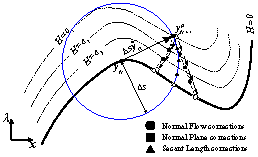
\includegraphics[scale=2.5]{FIG47.pdf}
	\caption{Two correction algorithms: Normal Flow and Normal Plane.}
	\label{fig:FIG47}
\end{figure}

Intermediate Normal Flow corrections correspond to
contours of $\bvec{H}$, $\bvec{H}_j$, where $\bvec{H}_j=\bvec{c}_{cont,j}$, 
$\Vert
\bvec{c}_{cont,j}\Vert_2>\epsilon_{tol}$, with $j$ the iteration counter. 
Normal Plane
corrections lie on a plane orthogonal to the tangent at $\bvec{y}_N$ and at
distance $\Delta s$, while Secant Length corrections are forced to lie on a
sphere of radius $\Delta s$, centered at $\bvec{y}_N$.

In any case, for the Augmented Jacobian approach,  $\bmat{B} = 
\bmat{A}^{-1}=[\bmat{DH}^T\ \ \bvec{q}_c]^{-1}$ and
$\bvec{r} = -[\bvec{H}^T\ \ V]^T$, where
$\dot{V}(\bvec{y})=\bvec{q}_c^T\dot{\bvec{y}}$.
The techniques derived from the Augmented Jacobian
approach underpin most incremental algorithms that have been developed 
for tackling stability problems in computational solid mechanics.
\cite{Wempner:1971,Riks:1972,Riks:1979,Crisfield3,Ramm:1981}. The Normal
Flow and two cases of Augmented Jacobian iterates are depicted in 
figure (\ref{fig:FIG47}), in particular the normal plane and secant length
methods. For details on the numerical linear algebra pertaining to these
methods, the interested reader can refer to the works of 
Keller\cite{Keller:1978,Keller:1983}, 
Chan and Keller\cite{ChanKeller:1982}, Griewank\cite{Griewank:1985},
Rheinboldt\cite{Rheinboldt:1983B}, Lin et.al.\cite{Lin:1987}, among others. 


%%%%%%%%%%%%%%%%%% APPENDIX G - GUI APP %%%%%%%%%%%%%%%%%%%%%%
\chapter{A Simple GUI for the Hybrid NLP Element}\label{appendix:APPENDIX_G}
%%%%%%%%%%%%%%%%%%%%%%%%%%%%%%%%%%%%%%%%%%%%%%%%%%%%%%%%%%%%%%%%%%%%%%%%%%%%


This chapter introduces a Graphical User Interface (\acrshort{gui}) developed 
as part of 
this work in order to 
facilitate analyses using the hybrid \acrshort{nlp} element. We detail the 
various features that are implemented using the AppDesigner utility of MATLAB, 
version 2022b. The chapter is divided in seven sections, each representing a 
particular tab of the interface. These seven tabs are : 1) Mesh, 2) Materials, 
3) Sections, 4) Boundary Conditions, 5) Analysis Controls, 6) Solve Job and, 
finally, 7) Post-processing. The first five tabs, some of which can be edited 
independently, belong to the pre-processing phase. Tab 6 calls the hybrid NLP 
solver for the given input in tabs 1-5 and tab seven provides post-processing 
infrormation with respect to the structure response in the form of 
force-displacement plots and  configuration history for all steps. A number of 
tooltips can be revealed by hovering over relevant fields.

\section*{The Mesh Tab}

The first tab of the \acrshort{gui}, depicted in Fig. \ref{fig:TAB1_marked}, is 
concerned 
with nodal and element input. We analyze it in terms of parts A to N:

\begin{itemize}
	\item \textbf{A}: The Mesh tab.
	\item \textbf{B}: Facility used to manually add nodes. Numeric values 
	pertaining to the X (horizontal) and Y (vertical) coordinate axes are used 
	in the corresponding fields to define the coordinates of a node. By 
	clicking on the \textit{Add Node} button, the enumerated node is added to 
	the table with its coordinated also listed. The enumeration is automatic. 
	Attempting to add a node with coordinates (X,Y) that are already defined 
	for another node results in an error, as shown in Fig. 
	\ref{fig:TAB1_node_error}.
	\item \textbf{C}: Facility used to delete a particular node. The 
	\textit{Label} field takes as input the node label already generated and 
	removes it from the table. The enumeration of remaining nodes is updated 
	accordingly. If node deletion is performed after the mesh is generated, the 
	latter is no longer valid and all elements are removed.
	\item \textbf{D}: Success/Error indicator of an action pertaining to node 
	generation, coupled with a text field for relevant message output (e.g. see 
	\ref{fig:TAB1_node_error}).
	\item \textbf{E}: Facility to generate a node set from a \textbf{.txt} or 
	\textbf{.xlsx} file. The format for this input file is shown in Fig. 
	\ref{fig:TAB1_nodesfile}. If a number of nodes have already been added 
	manually, this action replaces all existing nodes. In contrast, generating 
	a nodal set from an input file and then manually adding additional nodes 
	results in appending the previously generated nodal list.
	\item \textbf{F}: Table that lists all generated nodes along with their 
	coordinates.
	\item \textbf{G}: Facility used to manually add a (hybrid \acrshort{nlp}) 
	beam element. Since only one element per member is adquate with the 
	proposed formulation, the only relevant inputs are the start and end node 
	labels, indicated in the relevant fields as \textit{Node} $i$ and 
	\textit{Node} $j$ respectively. Again, adding an element with start and end 
	nodes already defined for an existing element results in an error. In 
	addition, element enumeration is, again, automatic.
	\item \textbf{H}: Element deletion facility. The element label used as 
	input in the relevant field and by clicking the \textit{Delete Element} 
	button results in removal of the particular element from the table. The 
	remainig elements are, again, automatically re-enumerated.
	\item \textbf{I}: Success/Error indicator of an action pertaining to 
	element generation, coupled with a text field for relevant message output.
	\item \textbf{J}: Facility to generate an element partition from a 
	\textbf{.txt} or \textbf{.xlsx} file. The format for this input file is 
	shown in Fig. \ref{fig:TAB1_elementsfile}. If a number of elements have 
	already been added manually, this action replaces all existing elements. In 
	contrast, generating an element partition from an input file and then 
	manually adding additional elements results in appending the previously 
	generated element list.
	\item \textbf{K}:  Table that lists all generated elements along with their 
	start and end nodes.
	\item \textbf{L}: Once clicked, the \textit{Clear Mesh} button resets all 
	existing input in the Mesh tab and the user can start over.
	\item \textbf{M}: \acrshort{gui} axes that dynamically update the existing 
	state of 
	nodal and mesh configuration. Figure \ref{fig:TAB1_mesh_example} shows the 
	Mesh tab when the mesh generation is complete for a simple case of a one 
	bay, one story frame. The nodal labels are places right next to their 
	respective nodes and are typeset in normal font while element labels are 
	approximately placed in the midspan of their corresponding elements and are 
	typeset in italic bold fonts.
	\item \textbf{N}: With the \textit{Load problem} facility, the user can 
	load a problem in its entirety. The appropriate file type is ASCII 
	(extension ".txt") and formatting details for the input file are discussed 
	in Section \ref{INPUTFILE} of this Appendix. Once the input file is 
	imported, the user 
	can go directly to tab \textit{Solve Job} and proceed with solving the 
	problem.
\end{itemize}

\begin{figure}
	\centering
	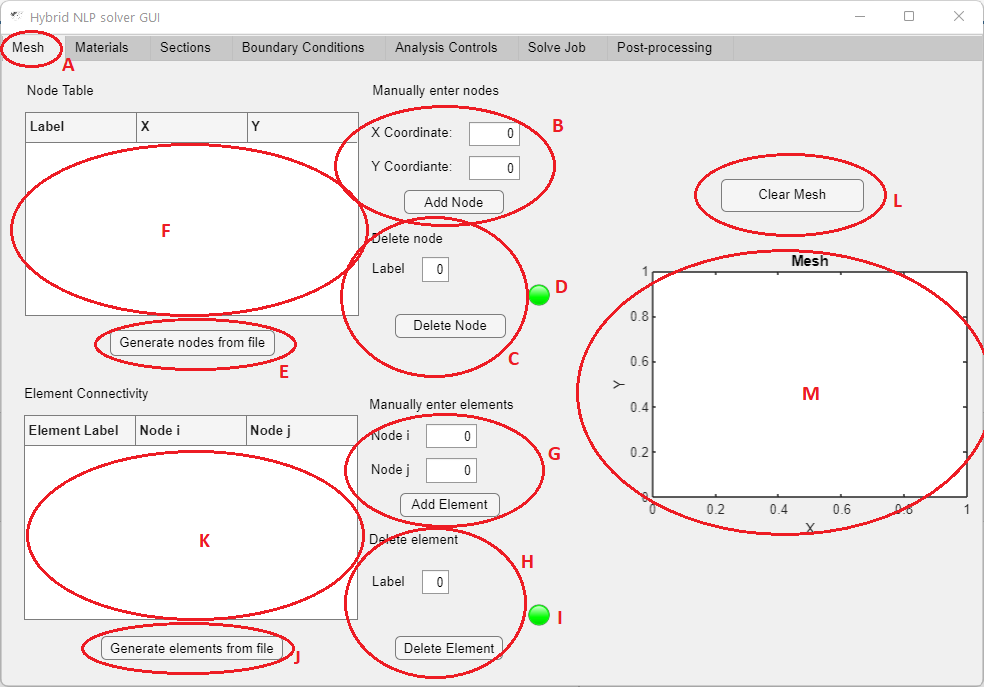
\includegraphics[scale=0.6]{GUIpics/TAB1/TAB1_marked.png}
	\caption{The \textit{Mesh} tab with relevant facilities A-M marked in red 
		circles 
		and enumerated with capital english letters.}
	\label{fig:TAB1_marked}
\end{figure}

\begin{figure}
	\centering
	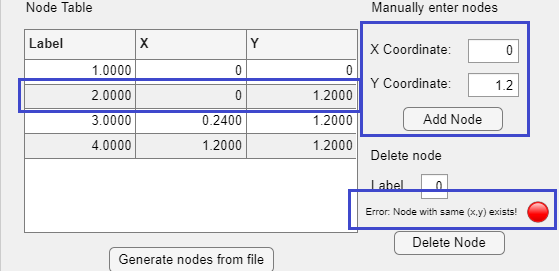
\includegraphics[scale=0.6]{GUIpics/TAB1/TAB1_node_error.png}
	\caption{Error when attempting to add a node with coordinates already 
		defined for an existing node.}
	\label{fig:TAB1_node_error}
\end{figure}

\begin{figure}
	\centering
	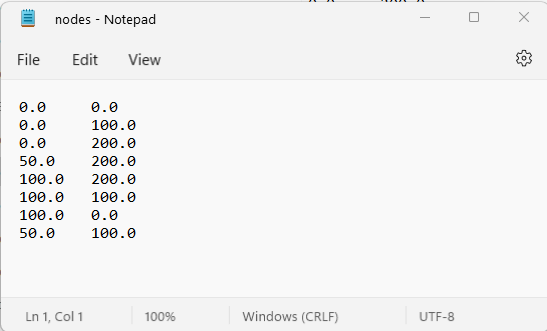
\includegraphics[scale=0.6]{GUIpics/TAB1/TAB1_nodesfile.png}
	\caption{A .txt file with the required format for nodal input. First column 
		is X coordinate, second is Y coordinate. The $k$-th row represents Node 
		$k$.}
	\label{fig:TAB1_nodesfile}
\end{figure}
\begin{figure}
	\centering
	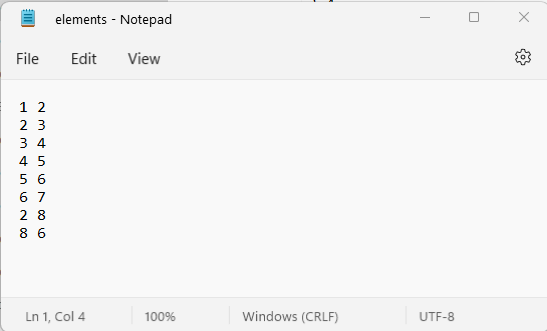
\includegraphics[scale=0.6]{GUIpics/TAB1/TAB1_elementsfile.png}
	\caption{A .txt file with the required format for element input. First 
		column is start node $i$, second is end node $j$. The $k$-th row 
		represents 
		Element $k$.}
	\label{fig:TAB1_elementsfile}
\end{figure}

\begin{figure}
	\centering
	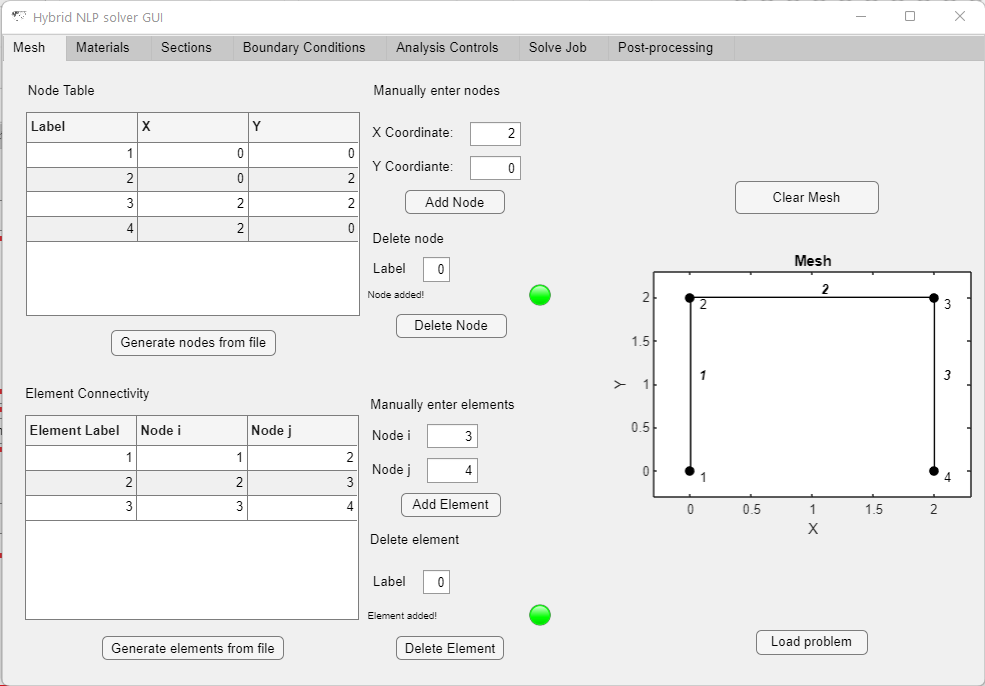
\includegraphics[scale=0.6]{GUIpics/TAB1/TAB1_mesh_example.png}
	\caption{The \textit{Mesh} tab with a completed mesh.}
	\label{fig:TAB1_mesh_example}
\end{figure}


\section*{The Materials Tab}

The \textit{Materials} tab follows the \textit{Mesh} tab and does not have any 
dependencies regarding previous input. Figure FIG outlines all relevant fields 
in this tab, again, separated by red cycles based on their functionality. We 
list and describe items A-I below:

\begin{itemize}
	\item \textbf{A}: The \textit{Materials} tab.
	\item \textbf{B}: Material name field. Takes alphanumeric values. If a 
	material name is not specified, a default name \textbf{Material}\_$\#$ is 
	used, where $\#$ takes values 1,2,3... etc. As an example, see Fig. 
	\ref{fig:TAB2_adding_mat_noname}.
	\item \textbf{C}: Numeric fields pertaining to elastic and plastic 
	properties of the material. In the case of purely elastic analysis, dummy 
	or zero values can be used in the plastic fields, as they are not 
	considered.
	\item \textbf{D}: The \textit{Add} and \textit{Delete} material facilities, 
	along with the Success/Error indicator (green lamp icon). To delete a 
	material defined previously, the user needs to click on it in the 
	\textit{Materials Panel} seen on the left side of the tab (\textbf{Item H}, 
	see below), and then click the \textit{Delete} button.
	\item \textbf{E}: Axes that depict the uniaxial stress-strain law for a 
	defined material. In order to activate it, the user will need to click on 
	the specific material in the \textit{Materials Panel} seen on the left side 
	of the tab (\textbf{Item H}, see below). An max strain 
	$\epsilon_{max}=10\epsilon_y$ is specified purely for plotting purposes. 
	This feature can be seen in Fig. \ref{fig:TAB2_materials_added}.
	\item \textbf{F}: The \textit{Update Material} facility updates the elastic 
	and plastic properties of an existing material. The material to be updated 
	needs to be selected in the \textit{Materials panel} seen on the left side 
	of the tab (\textbf{Item H}, see below). 
	\item \textbf{G}: A \textit{Standard materials} facility, which is 
	introduced to quickly add predefined, standardized materials from the 
	drop-down list. These materials are assumed to be elastic-perfectly plastic 
	but can be modified using the \textit{Update Material} facility. Two 
	materials are available: 1) Structural Steel(S235) and 2) Aluminum 
	Alloy(6062) (see Fig \ref{fig:TAB2_predefined_mats}). In contrast with 
	manually adding materials, duplicate 
	materials from the drop-down are not permitted, as can be seen from Fig. 
	\ref{fig:TAB2_adding_already_predefmat}. 
	\item \textbf{H}: This is the \textit{Materials} panel. All materials 
	defined and added are listed here. The user needs to click on a specific 
	material on the list in order to i) delete it, ii) update its parameters or 
	iii) view its uniaxial stress-strain plot.
	\item \textbf{I}: The elastic and plastic properties of a material selected 
	on the \textit{Materials} panel are shown in this table. The tabulated 
	quantities correspond to the material fields in \textbf{B} as follows:
	i) $E$ represents Young's modulus, ii) $\nu$ represents Poisson's 
	ratio, iii) f\_y represents the yield stress of the material, iv) 
	$H_{iso}$ represents the isotropic hardening modulus and v) $H_{kin}$ 
	represents the kinematic hardening modulus.
\end{itemize}

\begin{figure}
	\centering
	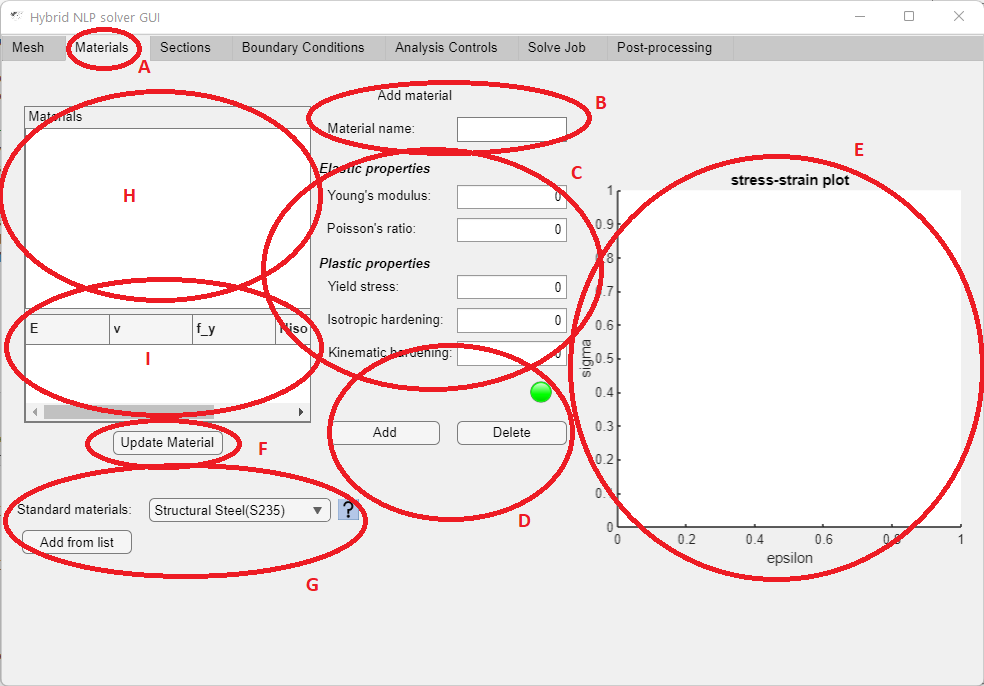
\includegraphics[scale=0.6]{GUIpics/TAB2/TAB2_marked.png}
	\caption{The \textit{Materials} tab with relevant facilities A-M marked in 
		red circles 
		and enumerated with capital english letters.}
	\label{fig:TAB2_marked}
\end{figure}


\begin{figure}
	\centering
	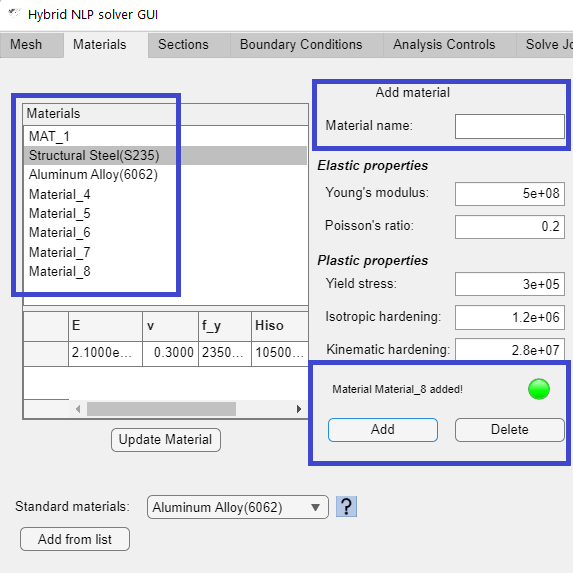
\includegraphics[scale=0.6]{GUIpics/TAB2/TAB2_adding_mat_noname.png}
	\caption{Multiple materials defined without a specified material name.}
	\label{fig:TAB2_adding_mat_noname}
\end{figure}

\begin{figure}
	\centering
	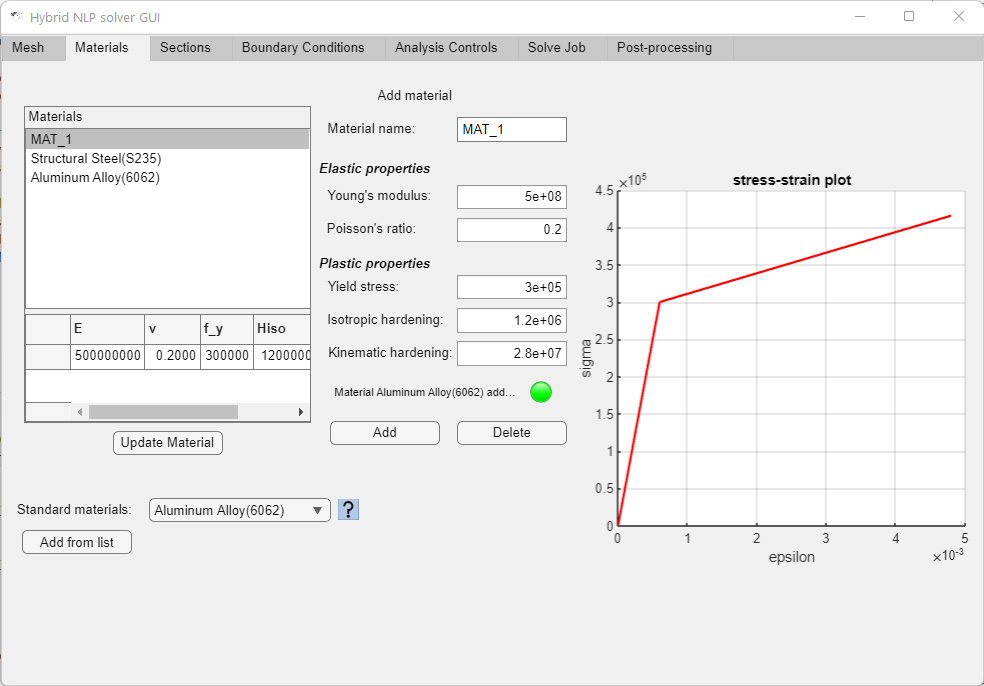
\includegraphics[scale=0.6]{GUIpics/TAB2/TAB2_materials_added.png}
	\caption{Potting of uniaxial stress-strain law of material \textbf{MAT}\_1.}
	\label{fig:TAB2_materials_added}
\end{figure}

\begin{figure}
	\centering
	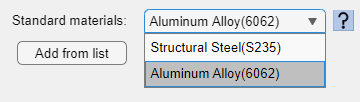
\includegraphics[scale=0.6]{GUIpics/TAB2/TAB2_predefined_mats.png}
	\caption{Available predefined materials from the \textit{Standard 
			materials} drop-down list.}
	\label{fig:TAB2_predefined_mats}
\end{figure}

\begin{figure}
	\centering
	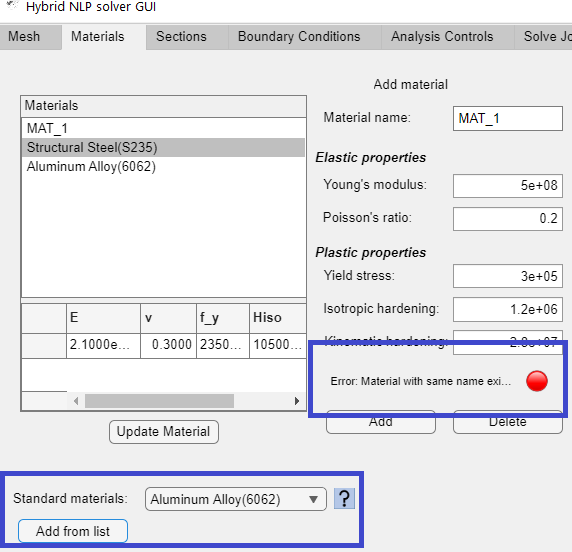
\includegraphics[scale=0.6]{GUIpics/TAB2/TAB2_adding_already_predefmat.png}
	\caption{Error when trying to add a standard material that was already 
		added previously.}
	\label{fig:TAB2_adding_already_predefmat}
\end{figure}

\section*{The Sections tab}

The third tab pertains to cross-section defintion. Cross-sections as objects 
are assigned a name, a shape, numeric values pertaining to the basic dimension 
of the selected shape (e.g. two basic dimensions for rectangular sections). 
Moreover, each section is assigned a material. As a consequence the 
\textit{Sections} tab has a dependency on the \textit{Materials} tab. If a  
material gets deleted, then all sections that were assigned that material get 
deleted as well. 

We now proceed with the description of the essential parts of the 
\textit{Sections} tab, shown in Fig. \ref{fig:TAB3_marked}.

\begin{itemize}
	\item \textbf{A}: The \textit{Sections} tab.
	\item \textbf{B}: Here, the user assign a name and a shape to the section. 
	The name field takes alphanumeric values. If not specified, then the name 
	\textbf{Section\_}$\#$ is assigned to the section, where $\# = 1,2,3, ...$. 
	The available shapes from the drop-down list are i) rectangular and ii) 
	(symmetric) wide flange geometries. 
	\item \textbf{C}: In this section, the user assigns numeric values to the 
	relevant fields that pertain to the basic dimensions of the assigned shape. 
	A rectangular shape has to basic dimensions: height $h$ and width $b$. The 
	wide flange shape has 2 additional shapes: web thickness $t_w$ and flange 
	thickness $t_f$. In addition, the user also specifies which material will 
	be assigned to the section. As can be seen from Fig. 
	\ref{fig:TAB3_section_added}, the section \textbf{Rectangular\_Section} is 
	assigned the material \textbf{MAT\_1} defined previously. The drop-down 
	list is also shown, where all other materials defined in the 
	\textit{Materials} tab are available in the list.
	\item \textbf{D}: Axes that depict the cross-section shape selected from 
	the drop-down list. The basic dimensions are also indicated in each case.
	\item \textbf{E}: In this part, the user assigns sections to elements. 
	Tapered element capabilities are not included in the present code, 
	therefore 
	only one section per element is permitted. A section is selected from the 
	\textit{Cross-Sections} panel, which is located at the top left of the tab 
	(see also \textbf{Item G} below) and then an element has to be selected 
	that will be assigned the section. Another feature for this part is the 
	capability to assign a specific to all elements, which is done by selecting 
	a section and then clicking on the \textit{Assign to all elements} button. 
	Lastly, a Success/Error indicator is included here as well in order to 
	facilitate the assignment process. For elements that are successfully 
	assigned a section, a message will be shown that states the name of the 
	assigned section, as shown in Fig. \ref{fig:TAB3_section_assigned} for 
	\textbf{Element 1} which was assigned the section 
	\textbf{Aluminum\_Section}. In contrast, for elements that have not been 
	assigned a section, when selected in the drop-down list, the indicator will 
	turn red and an appropriate message will be displayed. This can be seen in 
	Fig. \ref{fig:TAB3_NOsection_assigned}.
\end{itemize}

\begin{figure}
	\centering
	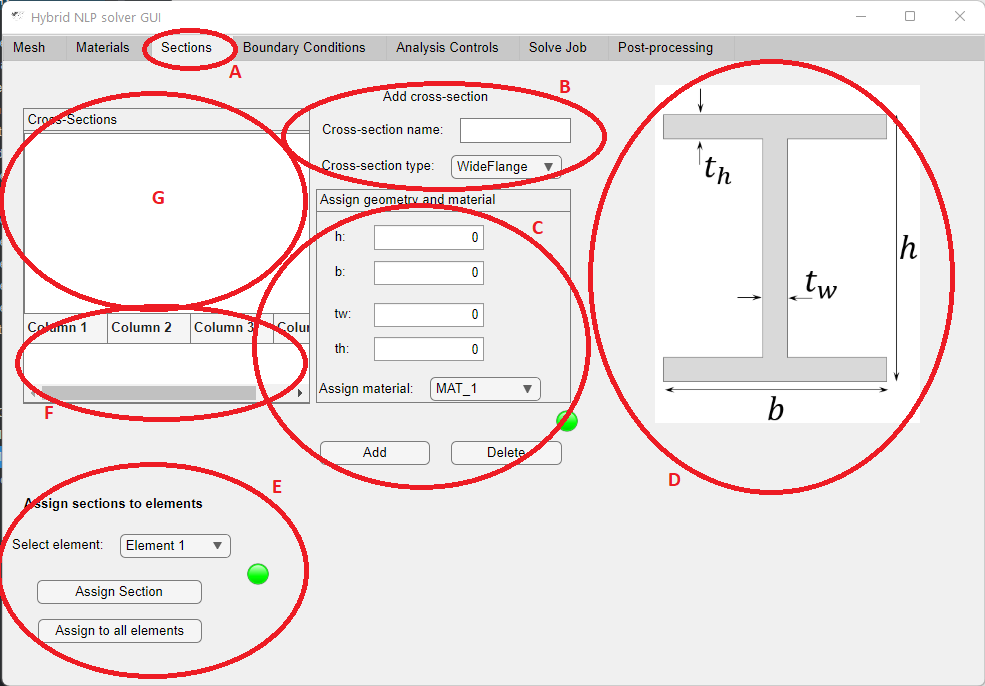
\includegraphics[scale=0.6]{GUIpics/TAB3/TAB3_marked.png}
	\caption{The \textit{Sections} tab with all essential parts marked in red 
		cycles and enumerated.}
	\label{fig:TAB3_marked}
\end{figure}

\begin{itemize}
	\item \textbf{F}: Table that lists the basic dimensions for the section 
	currently under selection in the \textit{Cross-Sections} panel (see below).
	\item \textbf{G}: The \textit{Cross-Sections} panel is where all sections 
	created are listed. In order to delete or assign a section to an element, 
	it has to be selected from the panel. 
\end{itemize}
\clearpage
\begin{figure}[t]
	\centering
	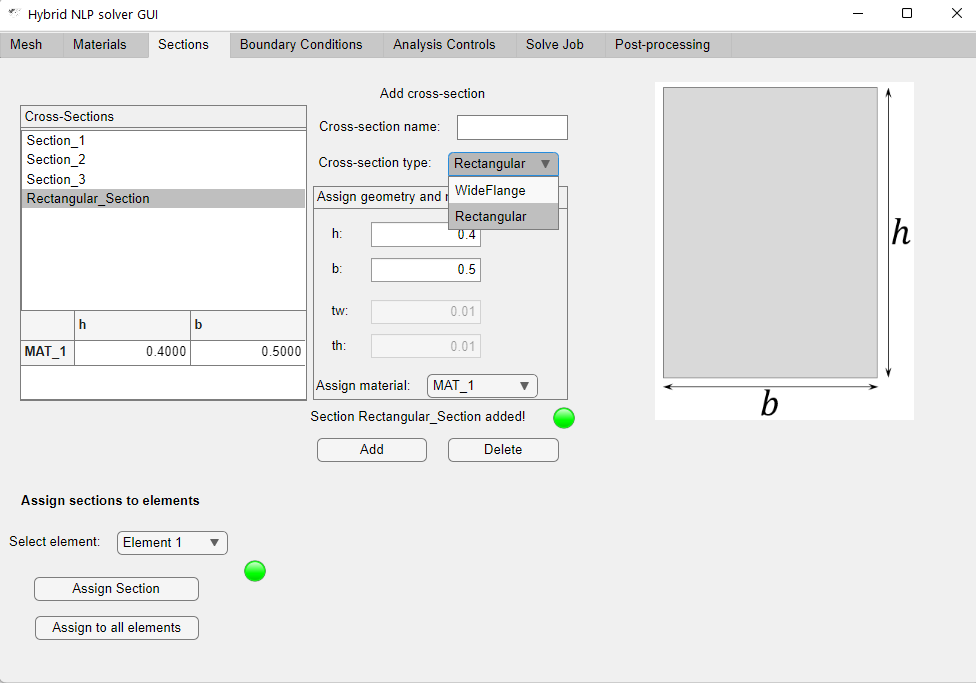
\includegraphics[scale=0.5]{GUIpics/TAB3/TAB3_section_added.png}
	\caption{Typical section definition process. A previously defined material 
		\textbf{MAT\_1} is assigned to section \textbf{Rectangular\_Section}.}
	\label{fig:TAB3_section_added}
\end{figure}

\begin{figure}[b]
	\centering
	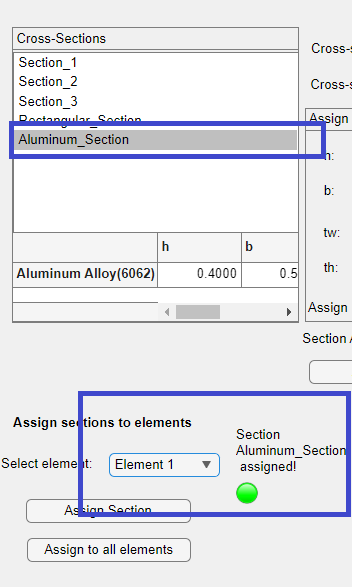
\includegraphics[scale=0.5]{GUIpics/TAB3/TAB3_section_assigned.png}
	\caption{Successful section assignment for \textbf{Element 1}.}
	\label{fig:TAB3_section_assigned}
\end{figure}
\clearpage
\begin{figure}
	\centering
	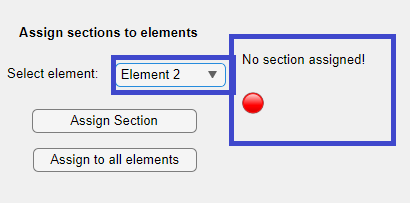
\includegraphics[scale=0.6]{GUIpics/TAB3/TAB3_NOsection_assigned.png}
	\caption{Indication that \textbf{Element 2} still needs to be assigned a 
		cross-section.}
	\label{fig:TAB3_NOsection_assigned}
\end{figure}

\section*{The Boundary Conditions tab}

In the \textit{Boundary Conditions} tab the user specifies the externally 
applied nodal loads \textit{and} and the nodal support conditions so that rigid 
body modes are excluded. The layout of the tab is shown in Fig. 
\ref{fig:TAB4_marked} and parts 
from A to F are discussed below:

\begin{itemize}
	\item \textbf{A}: The \textit{Boundary Conditions} tab.
	\item \textbf{B}: Here the user selects a node from the drop-down list at 
	the top to apply an external load at a certain nodal \acrshort{dof}. Once 
	the node is selected, the user can specify the magnitude and sign of the 
	applied force in three available force fields: 1) P1, which is aligned with 
	the global X axis (horizontal direction), 2) P2, which is aligned with the 
	global Y axis (vertical direction) and 3) M, which represents the moment 
	and the direction of the axis which it aligns with is determined by the 
	right-hand rule. In Fig. \ref{fig:TAB4_LOADS} an example is shown where 
	horizontal and vertical loads are applied at nodes 2 and 3.
	\item \textbf{C}: This is the \textit{Nodal Loads} table, where all nodes 
	that are assigned a non-zero external load along at least one nodal 
	\acrshort{dof} are listed (see \ref{fig:TAB4_LOADS}).
	
	\item \textbf{D}: Here, the user specifies supports conditions for certain 
	nodal \acrshort{dof}s. Again, after selecting a node from the drop-down 
	list, the user specifies which of the three available \acrshort{dof}s, U1, 
	U2 and U3, are fixed. There is a one-to-one correspondence between P1-P2-M 
	and U1-U2-U3 as far as direction of application. However, here, one only 
	needs to activate the available boxes in order to constrain the 
	corresponding displacement \acrshort{dof}. Figure \ref{fig:TAB4_SUPPORTS} 
	shows a case where node 1 is assigned a roller support condition (U1 and U2 
	fixed), whereas node 4 is assigned a clamp support condition (U1, U2, U3 
	fixed).
	\item \textbf{E}: Again, the table lists the nodes that have at least one 
	displacement \acrshort{dof} fixed (see Fig. \ref{fig:TAB4_SUPPORTS}).
	
	\item \textbf{F}: With the \textit{Clear} button, the user can erase all 
	input in this tab and start over.
\end{itemize}


\begin{figure}
	\centering
	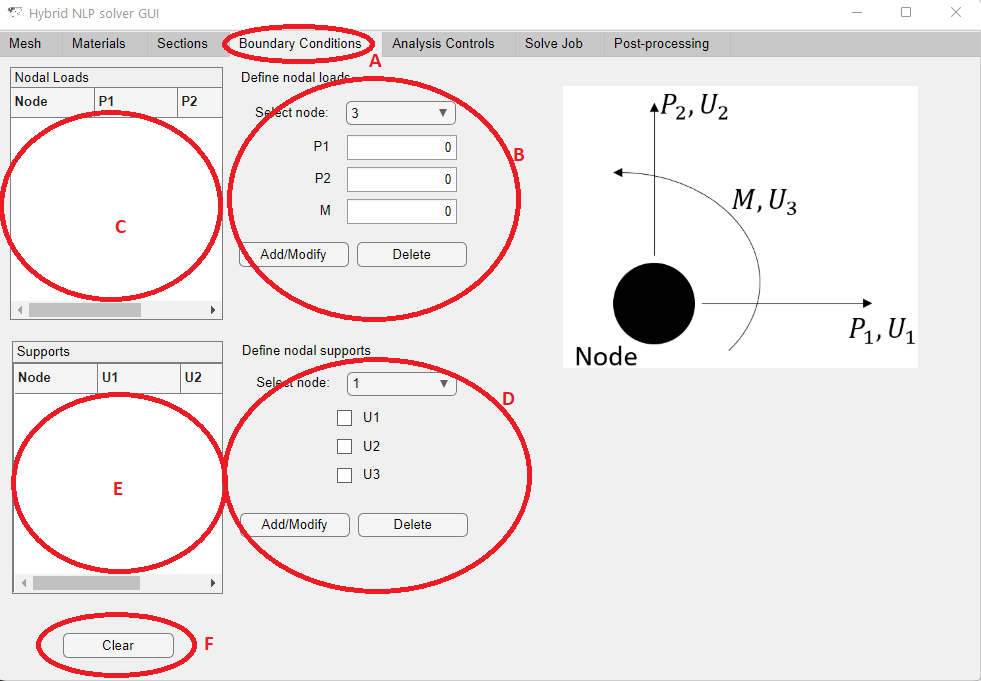
\includegraphics[scale=0.6]{GUIpics/TAB4/TAB4_marked.png}
	\caption{The \textit{Boundary Conditions} tab with all essential parts 
		marked in red cycles and enumerated.}
	\label{fig:TAB4_marked}
\end{figure}

\begin{figure}
	\centering
	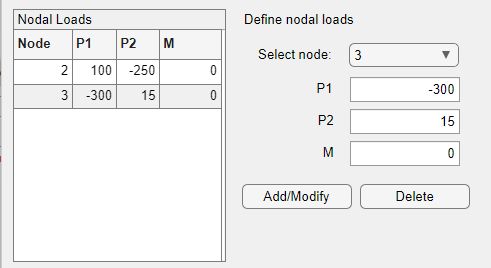
\includegraphics[scale=0.6]{GUIpics/TAB4/TAB4_LOADS.png}
	\caption{Input example for external nodal loading specification.}
	\label{fig:TAB4_LOADS}
\end{figure}

\begin{figure}
	\centering
	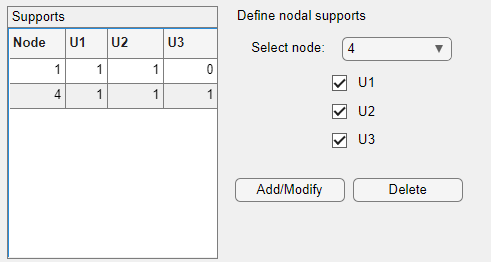
\includegraphics[scale=0.6]{GUIpics/TAB4/TAB4_SUPPORTS.png}
	\caption{Input example for nodal support specification.}
	\label{fig:TAB4_SUPPORTS}
\end{figure}

\section*{The Analysis Controls tab}

In the \textit{Analysis Controls} tab, the user can specify settings pertaining 
to geometric and constitutive assumptions as well as modify the default 
incremental analysis settings. An option to access advanced features is also 
given, whereby one can select between different continuation solvers and, if 
the Homotopy solver is chosen, the user can further specify details such as 
prediction and correction schemes. The latter gives the option to use the 
\acrshort{wls} predictor. 

The basic layout of the tab is shown in Fig. \ref{fig:TAB5_marked}. The marked 
components are:

\begin{itemize}
	\item \textbf{A}: The \textit{Analysis Controls} tab.
	\item \textbf{B}: The option to enable geometrically-exact kinematic 
	assumptions. When it is, the equilibrium solver used by default is 
	Crisfield's cylindrical arc-length method. For this reason, the user can 
	also specify a step-length, $DS$. 
	\item \textbf{C}: This option pertains to the incorporation of material 
	nonlinearities during the analysis. It is disabled by default. If enabled, 
	the user can also specify the number of cross-section layers. This number 
	is the same for all sections in the structure.
	\item \textbf{D}: Option that pertains to the incorporation shear effects 
	during the analysis. If enabled, which is the default setting, and the 
	plastic analysis option is also enabled, then a quadratic distribution for 
	the shear strains is assumed along the cross-section height.
	\item \textbf{E}: Numerical quadrature options. The user can choose between 
	Gauss-Legendre and Gauss-Lobatto schemes. The latter tends to be more 
	accurate for frame structures since the end-points of the domain are 
	included in the quadrature set.
	\item \textbf{F}: The user sets the order of numerical quadrature. The 
	minimum allowed is 1 and the maximum is 12.
	\item \textbf{G}: Number of incremental steps to be used if the Load 
	Control equilibrium solver is chosen. When the Cylindrical arc-length is 
	used, this number simply divides the external load vector in order to get a 
	base load.
	\item \textbf{H}: Maximum number of steps. It pertains only to continuation 
	solvers, such as Crisfield's Cylindrical arc-length and the Homotopy 
	solver. The solver will stop 1) when the external load is surpassed or 2) 
	when the maximum number of steps is reached.
	\item \textbf{I}: The maximum number of correction iterations to be 
	performed during an incremental step.
	\item \textbf{J}: The tolerance used to test convergence in term of the 
	Euclidian norm of the out-of-balance (residual) force vector.
	\item \textbf{K}: Option to show the advanced analysis settings (see below).
	\item \textbf{L}: Once the user has specified all analysis controls in tab, 
	they have to register the input by clicking on the \textit{Register 
		changes} button.
	\item \textbf{M}: The user can reset all settings in this tab to their 
	defaults by using the \textit{Reset to defaults} button.
	\item \textbf{N}: Success/Error indicator for this tab.
\end{itemize}

We now discuss the advanced settings panels, shown in Fig. 
\ref{fig:TAB5_marked_advanced}, which become visible only when the 
\textit{Advanced settings}(\textbf{K}) option is enabled:

\begin{itemize}
	\item \textbf{O}: Drop-down list (see Fig. \ref{fig:TAB5_solvers}) where 
	the user can select between three different solution schemes: 1) Load 
	Control, 2) Crisfield's arc-length and 3) Homotopy solver. By default, 
	Crisfield's solver is enabled. 
	\item \textbf{P}: Numeric fields pertainig to a) minimum step-length, b) 
	maximum step-length and c) step-length adjustment parameter. The first two 
	limits ensure that the step-length will not become exceedingly small or 
	large. The latter adjust the step-length based on how easily the solution 
	process converged in the last step. It is advised that, in case of plastic 
	analyses, parameter $a$ be set to values between 4 and 8. These three 
	options are not relevant to the Load Control scheme. The values shown in 
	Fig. \ref{fig:TAB5_marked_advanced} are the default ones.
	\item \textbf{Q}: Option to force Crisfield's arc-length and the Homotopy 
	solver to repeat the last incremental step until the reach load is within a 
	specified tolerance of the externally applied load. If this option is not 
	enabled the solver will stop when the base load mulitplied by the load 
	factor simply exceed the external load vector.
	\item \textbf{R}: Option that, when enabled, forces the Homotopy and 
	Crisfield's arc-length solvers to repeat steps that failed to converge 
	within the specified iteration counter, but with halved step-length. The 
	same step will be repeated until convergence or the min$DS$ is reached.
	\item \textbf{S}: The options in the \textit{Homotopy solver settings} 
	become visible only when the Homotopy solver is selected in \textbf{O}. The 
	Predictor option allows the user to choose between i) tangent differential 
	predictor and ii) the \acrshort{wls} predictor. If the latter is chosen, an 
	additional panel of options, specific to this precition scheme, appears.
	\item \textit{T}: Here the user can specify the correction scheme to be 
	used. The three options are: i) Normal Flow\cite{Watson:1989}, ii) 
	Secant-Length\cite{Schwetlick87} and iii) Normal Plane\cite{Riks:1979}.
	
	\item \textbf{U}: If the \textit{WLS predictor} is selected in \textbf{S}, 
	the user can specify which variant of the \acrshort{wls} predictor to use. 
	The available options are: i) \acrshort{wlse}, which is the default, ii) 
	\acrshort{wlst} and iii) \acrshort{wlsit}.
	\item \textbf{V}: This parameter determines the number of load-controlled 
	steps to be performed before the homotopy solver using \acrshort{wls} 
	predictor takes over. A number of simple Newton steps need to be performed 
	in order to generate enough solutions available for the \acrshort{wls} 
	scheme.
	\item \textbf{m}: The degree of polynomial basis used in the \acrshort{wls} 
	fitting. In this version, this remains constant throughout the analysis. 
	Future versions will provide an option to automatically adjust it during 
	the solution process.
	\item \textbf{N0}: The number of previously converged points to consider 
	for the \acrshort{wls} fitting. In this version, this remains constant 
	throughout the analysis. Future versions will provide an option to 
	automatically adjust  it during the solution process.
	\item \textbf{beta}: The weight function parameter, with default value 0.2. 
	If set to 1, then there is no weighting during the least squares fitting. 
	Keep this parameter larger than zero.
\end{itemize}
\begin{figure}
	\centering
	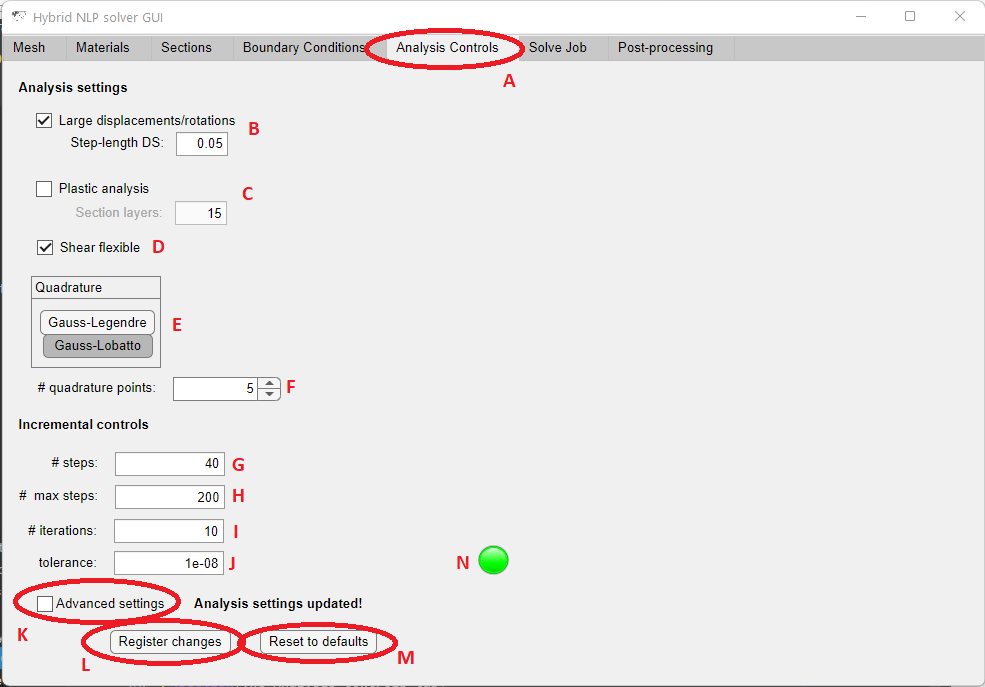
\includegraphics[scale=0.6]{GUIpics/TAB5/TAB5_marked.png}
	\caption{The \textit{Analysis Controls} tab with all essential parts 
		marked in red cycles and enumerated.}
	\label{fig:TAB5_marked}
\end{figure}

\begin{figure}
	\centering
	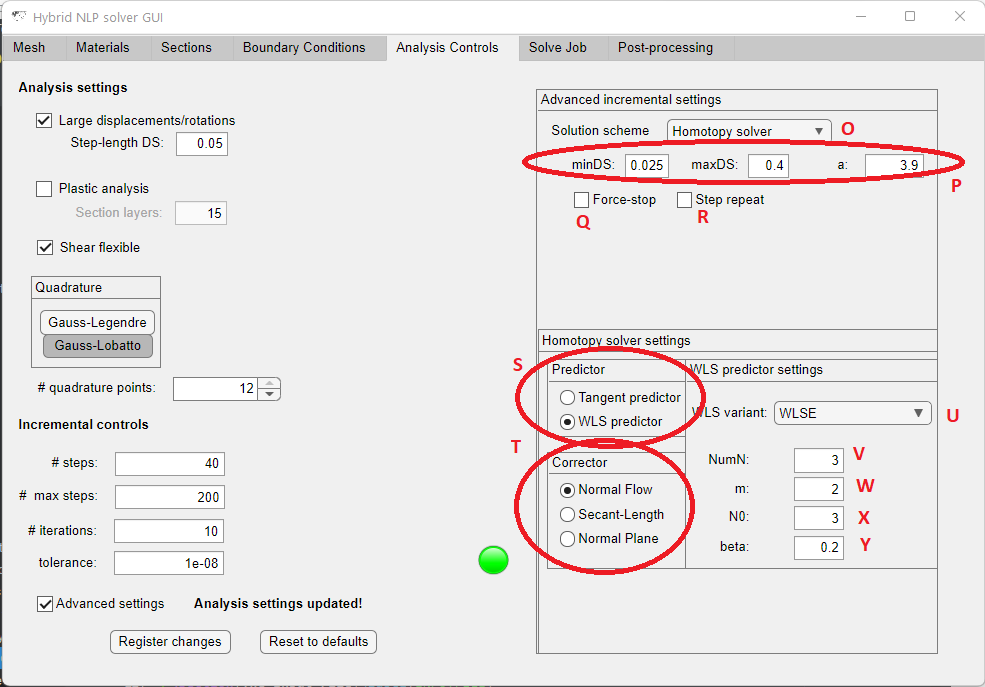
\includegraphics[scale=0.6]{GUIpics/TAB5/TAB5_marked_advanced.png}
	\caption{The \textit{Analysis Controls} tab with the advanced settings 
		enabled.}
	\label{fig:TAB5_marked_advanced}
\end{figure}

\begin{figure}
	\centering
	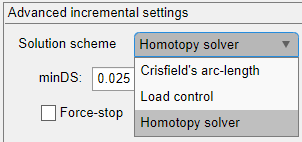
\includegraphics[scale=0.6]{GUIpics/TAB5/TAB5_solvers.png}
	\caption{The \textit{Analysis Controls} tab with the advanced settings 
		enabled.}
	\label{fig:TAB5_solvers}
\end{figure}

\section*{The Solve Job tab}

This is the tab where input, if successfully registered, is submitted and the 
structural problem is solved using the hybrid \acrshort{nlp} element. The 
layout, shown in Fig. FIG, is fairly simple and relevant parts are:

\begin{itemize}
	\item \textbf{A}: The \textit{Solve Job} tab.
	\item \textbf{B}: If all imput is successfully registered, then clicking on 
	the \textit{Solve Job} button will call the hybrid \acrshort{nlp} solver. 
	Otherwise, an error message will be shown and the user will be directed to 
	the relevant tab to make corrections.
	\item \textbf{C}: The text box where all analysis settings specified by the 
	user are displayed once the job is submitted. When the analysis is over, 
	the number of steps and total iterations is also displayed.
\end{itemize}


\begin{figure}[t]
	\centering
	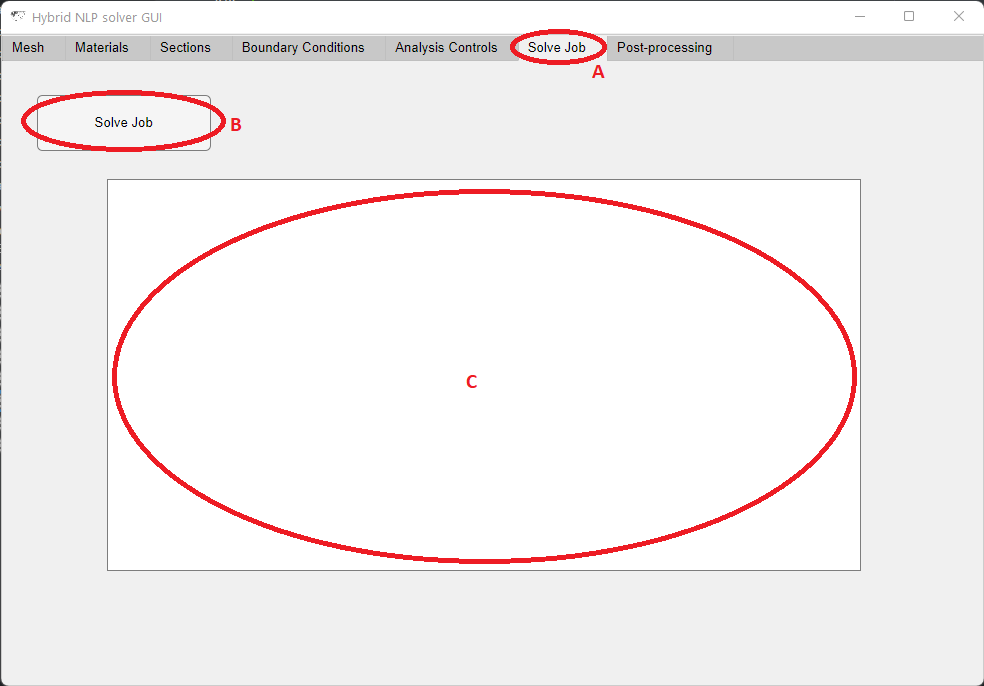
\includegraphics[scale=0.5]{GUIpics/TAB6/TAB6_marked.png}
	\caption{The \textit{Solve Job} tab.}
	\label{fig:TAB6_marked}
\end{figure}

\clearpage

\section*{The Post-processing tab}

In the \textit{Post-processing} tab the user can choose to plot i) load - 
displacement equilibrium paths for selected \acrshort{dof}s and ii) the 
deformation history of the structure. The tab layout is shown in Figs. 
\ref{fig:TAB7_markedA}, \ref{fig:TAB7_markedB}, and tab layout, along with the 
panels pertaining to \textit{Equilibrium path} and \textit{Deformation 
	history}, are discussing below:

\begin{itemize}
	\item \textbf{A}: The \textit{Post-processing} tab.
	\item \textbf{B}: The \textit{Equilibrium path} panel.
	\item \textbf{C}: The \textit{Deformation history} panel.
	\item \textbf{D}: Here, the user selects a node from the drop-down list and 
	a displacement \acrshort{dof} for the (horizontal) X-axis from the 
	\textit{Nodal DOF} button group.
	\item \textbf{E}: Here, in a similar fastion with \textbf{D}, the user 
	selects a node from the drop-down list and a \acrshort{dof} from the button 
	group to the right where an external load is specified with non-zero value. 
	The force will be assigned to the (vertical) Y-axis.
	
	\item \textbf{F}: In these three text fields, the user specifies the labels 
	for X and Y axis and the title for the plot.
	
	\item \textbf{G}: Here, the user specifies the color of the equilibrium 
	curve. The color format follows native MATLAB rules.
	\item \textbf{H}: In this (text) field, the user specifies the linestyle of 
	the equilibrium curve. This, again, follows standard MATLAB formatting 
	rules. For example, a dashed line is specified as "--", a line with cycle 
	markers as "-o" etc.
	
	\item \textbf{I}: Once activated, the \textit{Plot equilibrium path} button 
	plots the equilibrium path for the selected \acrshort{dof}s.
	\item \textbf{J}: Once the \textit{Clear figure} button is activated, it 
	clears the figure in the present tab.
	\item \textbf{K}: Option to export the current plot. The user can specify a 
	name in the text field \textit{Filename} and a filetype from the 
	\textit{Extension} drop-down list. The available extensions are: ".pdf" and 
	".fig", which exports the plot as a MATLAB figure.
	\item \textbf{L}: The embedded axes for this tab where graphic objects are 
	displayed.
	
\end{itemize}

\begin{figure}
	\centering
	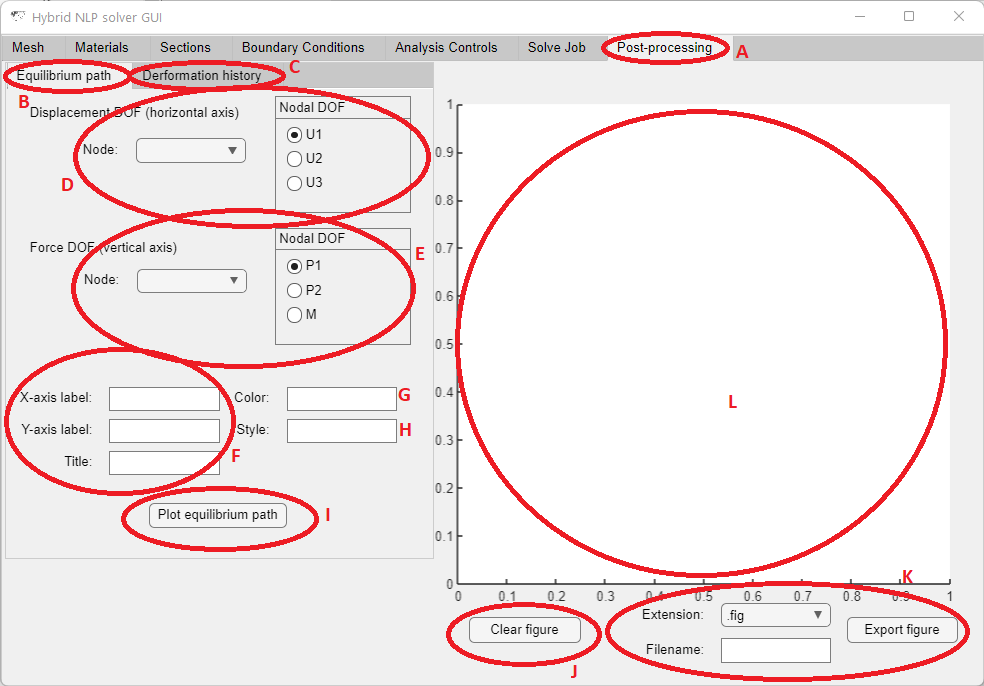
\includegraphics[scale=0.6]{GUIpics/TAB7/TAB7_markedA.png}
	\caption{The \textit{Post-processing} tab and the \textit{Deformation 
			history} panel.}
	\label{fig:TAB7_markedA}
\end{figure}

\begin{itemize}
	\item \textbf{M}: The \textit{Animate} button in the \textit{Deformation 
		history} panel (see Fig. \ref{fig:TAB7_markedB}) generates all the 
	necessary data in order to produce a deformation history animation for the 
	structure. This may take a while in case a plastic analysis or a small 
	step-length general nonlinear analysis is performed. Once the deformation 
	data have been generated, the \textit{Animate} button can be used again to 
	produce the same animation but without repeating the costly post-processing 
	calculations.
	
	\item \textbf{N}: Slider that can be used to contrast intermediate 
	configuration states for the structure, compared to the last one, which is 
	the last frame produced by the animation. The slider is not enabled when 
	the deformation data have not been produced. 
\end{itemize}

\begin{figure}
	\centering
	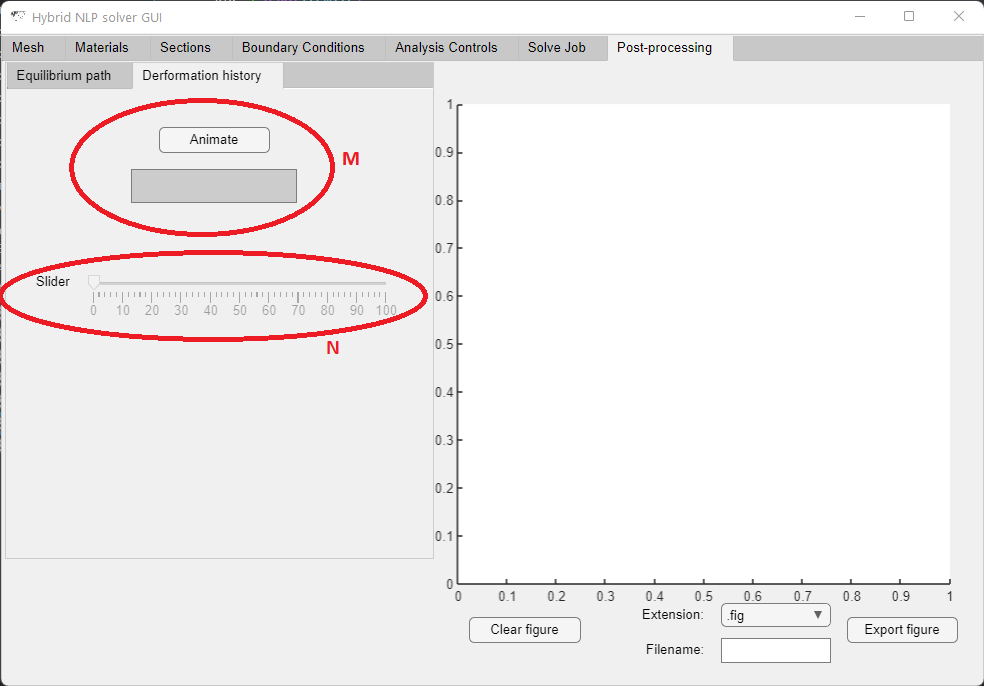
\includegraphics[scale=0.6]{GUIpics/TAB7/TAB7_markedB.png}
	\caption{The \textit{Solve Job} tab and the \textit{Deformation history}.}
	\label{fig:TAB7_markedB}
\end{figure}

Plotting using these two utilities are shown in Figs. \ref{fig:TAB7_EQPLOT}, 
\ref{fig:TAB7_slider}. Figure \ref{fig:TAB7_EQPLOT} shows the equilibrium path 
for U2 at node 3 against P2 again at node 3. Figure \ref{fig:TAB7_slider} on 
the other hand shows the final configuration of Lee's Frame along with the 
configuration at step 12, which is retrieved using the slider utility.

\begin{figure}
	\centering
	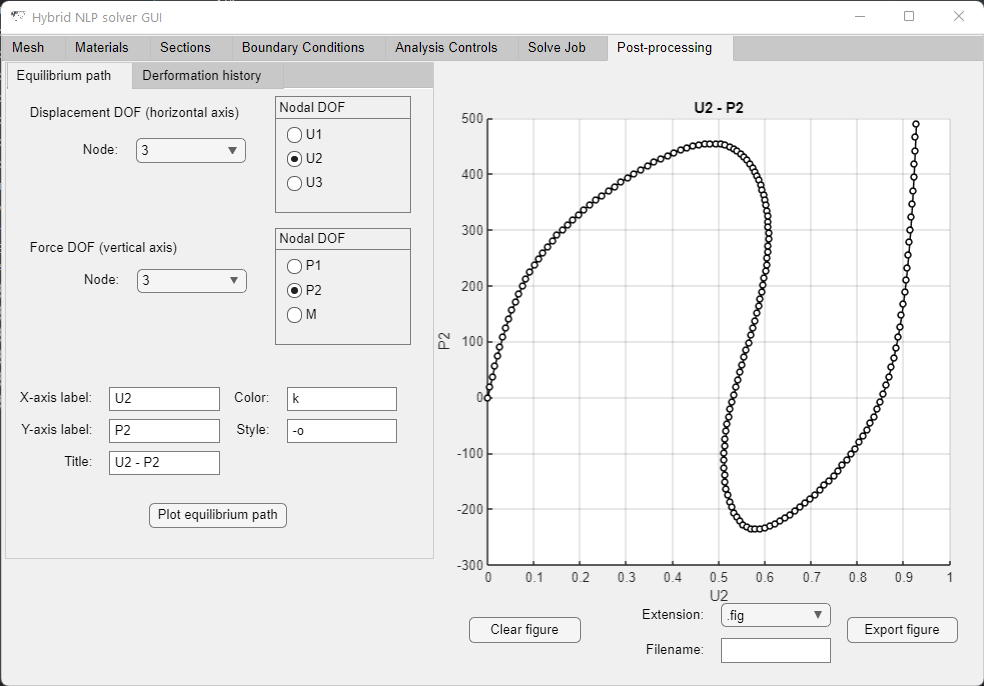
\includegraphics[scale=0.6]{GUIpics/TAB7/TAB7_EQPLOT.png}
	\caption{Equilibrium path plot.}
	\label{fig:TAB7_EQPLOT}
\end{figure}

\begin{figure}
	\centering
	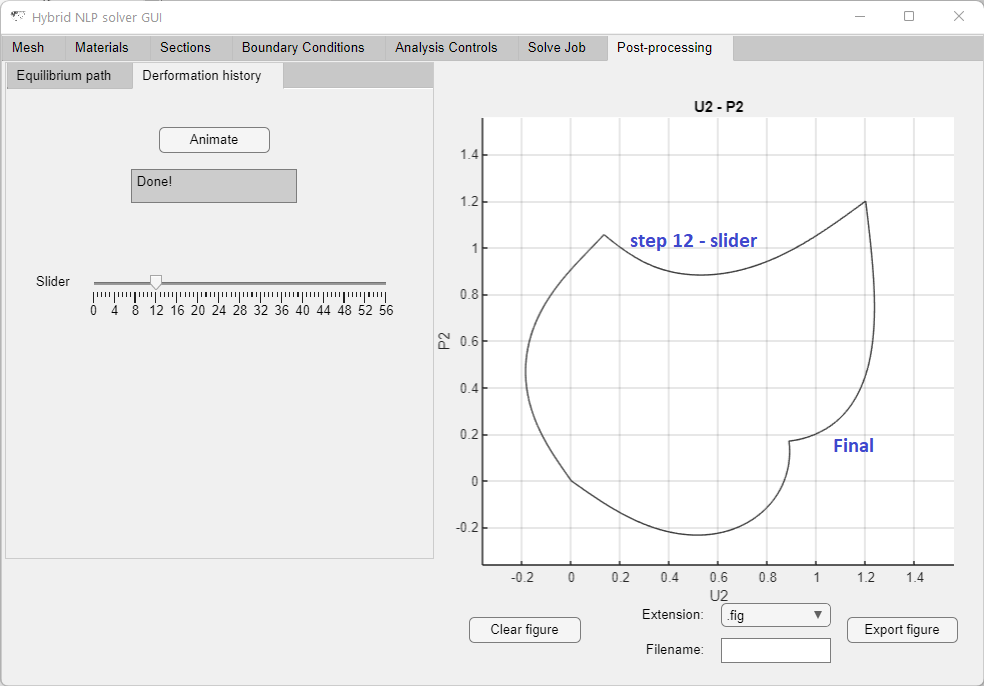
\includegraphics[scale=0.6]{GUIpics/TAB7/TAB7_slider.png}
	\caption{Deformation history plot of the structure.}
	\label{fig:TAB7_slider}
\end{figure}

\section*{The Input File}\label{INPUTFILE}

We now discuss the structure of the input file and how the application parses 
its contents. We highlight again that the input file contains all data required 
to run an analysis for a particular structure: mesh, materials, cross-sections 
and element-section assignments, boundary conditions and analysis controls.

The input file is imported using the \textit{Load problem} found in the 
\textit{Mesh} tab, which is highlighted in the figure below:

\begin{figure}
	\centering
	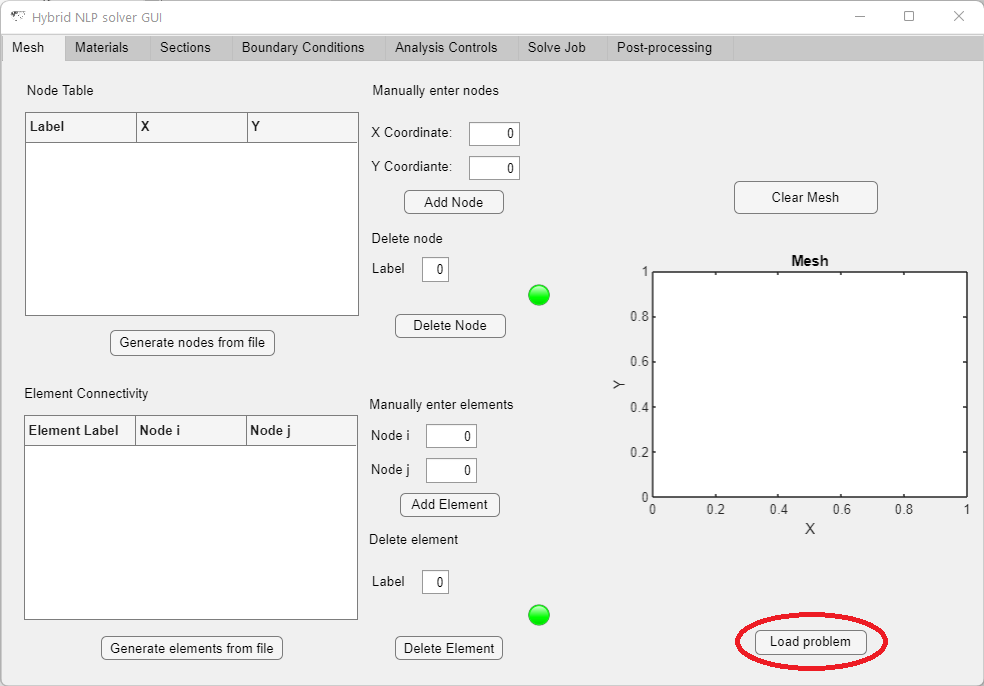
\includegraphics[scale=0.6]{GUIpics/INPUT_FILE/IMAGE_1.png}
	\caption{Load problem using the input file.}
	\label{fig:IMAGE_1}
\end{figure}

The input file consists of seven sections or parts and are separated by ".,", 
parsing the file from top to bottom. Each part pertains to a certain category 
of inputs. The categories of inputs are listed below and they have to follow 
this hierarchy:

\begin{enumerate}
	\item NODES
	\item ELEMENTS
	\item MATERIALS (6 inputs per material, repeat input for additional 
	materials)
	\item SECTIONS (7 inputs per section, repeat input for additional sections)
	\item ELELEMT-SECTION ASSIGNMENTS
	\item BOUNDARY CONDITIONS
	\item ANALYSIS CONTROLS (25 inputs in total)
\end{enumerate}

The input file is loaded and converted into a MATLAB Cell data structure. 
Inputs that require more than one numeric value, such as nodal coordinates for 
a node, should be separated by a comma. The use of commas results in a cell 
structure with columns, where a new column starts after a comma. Lines that 
start with "$\#$" are treated as comments and are 
ignored by the parser. In addition, different sections are assigned different 
``widths", where width is to be understood as the number of columns the data 
for a particular section span. For example, the NODE and ELEMENTS input 
sections require two columns, therefore the parser will ignore anything written 
after the second column for these two sections. For the MATERIALS or SECTIONS 
parts, only one column suffices and therefore, comments in these parts can 
start at the second column. For the BOUNDARY CONDITIONS part we need four 
columns, that is, the node label and values at the three \acrshort{dof}s at 
that node. Therefore, the parser will start ignoring input after the fourth 
column in that section. 

\subsection*{The NODE input}

An example of nodal coordinate input on the ASCII input file and how it is 
stored into a MATLAB cell is shown in Fig. \ref{fig:NODE}. As can be seen from 
that figure, the NODE part requires two numeric values per line, where a line 
represents a node: a X and a Y coordinate, which correspond to the first and 
second column respectively and are seperated by commas. When the nodal input is 
finalized, the dot character followed by a comma, ".," should be added in the 
next line. This tells the parses that nodal input is over and the ELEMENTS 
input is next.


\begin{figure}
	\centering
	\subfloat[ASCII file 
	formatting.]{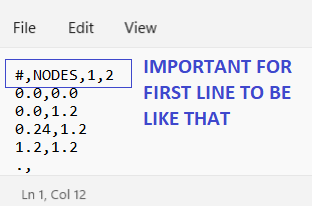
\includegraphics[width=0.5\textwidth]{GUIpics/INPUT_FILE/NODE_TXT.png}
		\label{fig:NODEA}}
	
	\subfloat[MATLAB Cell 
	storage.]{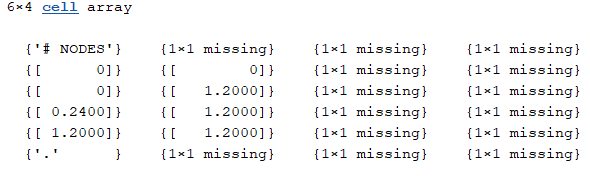
\includegraphics[width=0.5\textwidth]{GUIpics/INPUT_FILE/NODE_MAT.png}}
	
	\caption{How NODE part is typeset in the ASCII file and how it is stored in 
		a cell data structure by MATLAB.}
	\label{fig:NODE}
\end{figure}

Note the way the first line is typeset in \ref{fig:NODEA}. It is crucial  that 
the first line in the input file starts with the comment character $\#$ and 
also includes at least 4 commas. This is done in order to ensure that MATLAB 
will store all data in a cell with \textbf{at least four columns}.

\subsection*{The ELEMENTS input}
Like the NODE part, the ELEMENT input takes two numeric values per line 
(element), which correspond to nodes $I$ and $J$ that the element connects. The 
relevant portion of the ASCII file is shown in Fig. \ref{fig:ELEMENTS}.

\begin{figure}
	\centering
	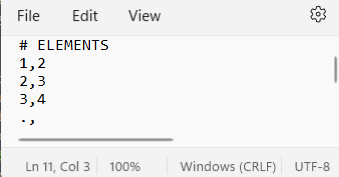
\includegraphics{GUIpics/INPUT_FILE/ELEMENT_TXT.png}
	\caption{How ELEMENTS part is typeset in the ASCII file.}
	\label{fig:ELEMENTS}
\end{figure}

\subsection*{The MATERIALS input}
In this part the user defines a list of materials. Only one column is required 
and 6 parameters define a material completely. Multiple materials can be 
defined by repeating the sequence of MATERIALS input, as shown in Fig. 
\ref{fig:MATS} for three materials. The order in which the material parameters 
are defined needs to be the same as shown in pictures: 
\begin{enumerate}
	\item Material Name (String type)
	\item Young's modulus (Numeric type)
	\item Poisson's ratio (Numeric type)
	\item Yield stress (Numeric type)
	\item Isotropic Hardening modulus (Numeric type)
	\item Kinematic Hardening modulus (Numeric type)
\end{enumerate}

\begin{figure}[t]
	\centering
	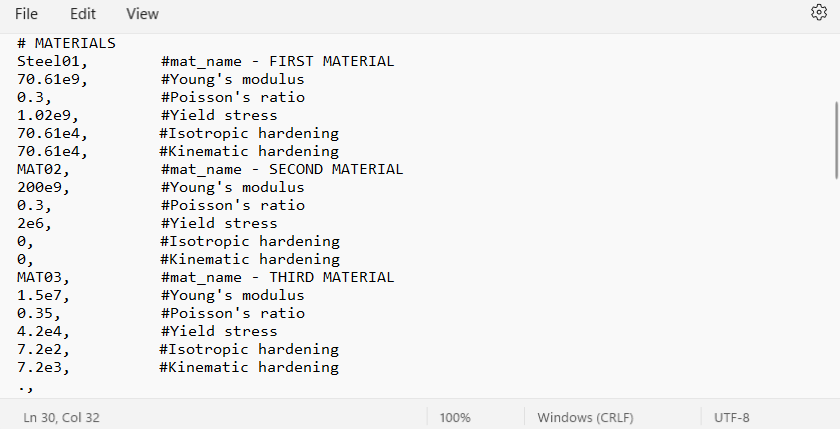
\includegraphics[scale=0.75]{GUIpics/INPUT_FILE/MATS_TXT.png}
	\caption{How MATERIALS part is typeset in the ASCII file, with multiple 
		materials defined.}
	\label{fig:MATS}
\end{figure}

\subsection*{The SECTIONS input}

Sections are defined in a similar fashion to materials. One section is 
completely determined by seven parameters which are detailed below and have to 
be defined in the same order when they are typeset in the ASCII file:

\begin{enumerate}
	\item Section Name (String type)
	\item Cross-section identifier (Numeric type, 1:Symmetric wide flange or 
	2:Rectangular)
	\item Cross-section height (Numeric type)
	\item Cross-section width (Numeric type)
	\item Web thickness (Numeric type)
	\item Flange Thickness (Numeric type)
	\item Assigned Material (String type)
\end{enumerate}

In the case where a Rectangular section is defined, the web and flange 
thicknesses can be assigned dummy values. Again, multiple sections can be 
defined by repeating the above sequence of parameters. An example where three 
cross-section are define in the SECTIONS part is shown in Fig. \ref{fig:SECS} 
below.

\begin{figure}[t]
	\centering
	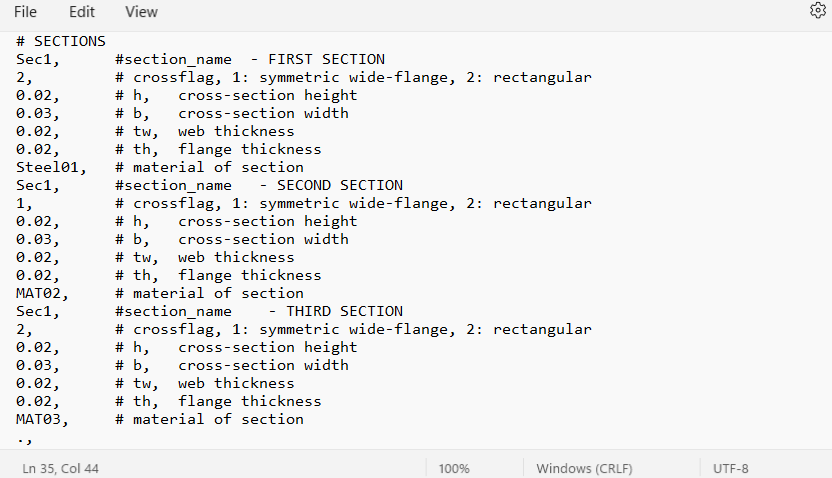
\includegraphics[scale=0.75]{GUIpics/INPUT_FILE/SECS_TXT.png}
	\caption{How SECTIONS part is typeset in the ASCII file, with multiple 
		cross-sections defined.}
	\label{fig:SECS}
\end{figure}


\subsection*{The ELEMENT-SECTION ASSIGNMENT input}

Here the user specifies couples that encapsulate information regarding 
cross-section assignment to elements. The first input in the couple, and by 
extension elements in the first column, is the element label, which is 
represented by an integer. The second input in the couple is the cross-section 
name, which is stored in a variable of type "string". Evidently, the number of 
rows dedicated to this input section should match the number of elements 
defined previously. The input template for assigning sections to elements is 
shown in Fig. \ref{fig:ELESECS} below.

\begin{figure}[t]
	\centering
	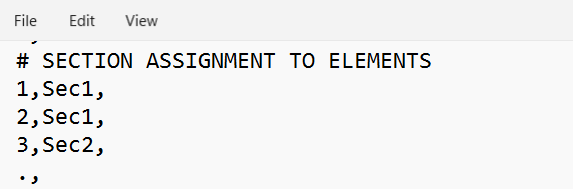
\includegraphics[scale=0.75]{GUIpics/INPUT_FILE/ELESEC_TXT.png}
	\caption{The ELEMENT-SECTION ASSIGNMENT input block.}
	\label{fig:ELESECS}
\end{figure}

\subsection*{The BOUNDARY CONDITION input}

In this part, the user first specifies the loading boundary conditions and then 
the displacement ones. The two blocks are separated by the dot/comma character 
".," as is done for normal input sections. Four entries are required to fully 
define a boundary condition: a node label, which is a positive integer, and 
three values corresponding to the three \acrshort{dof}s at that node. Figure 
\ref{fig:BCS} shows an example where Node 3 is assigned a vertical downward 
load and rollers are assigned to Nodes 1 and 4.

\begin{figure}[t]
	\centering
	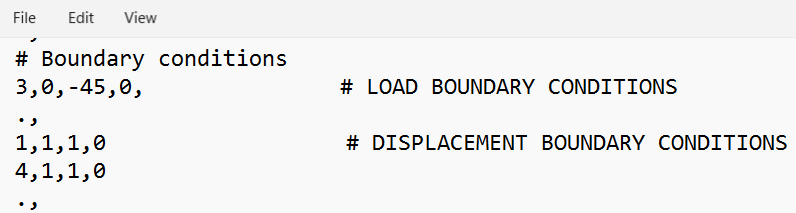
\includegraphics[scale=0.75]{GUIpics/INPUT_FILE/BCS_TXT.png}
	\caption{Defining load and displacement boundary conditions in the BOUNDARY 
		CONDITIONS block for the ASCII input file.}
	\label{fig:BCS}
\end{figure}

\begin{figure}[t]
	\centering
	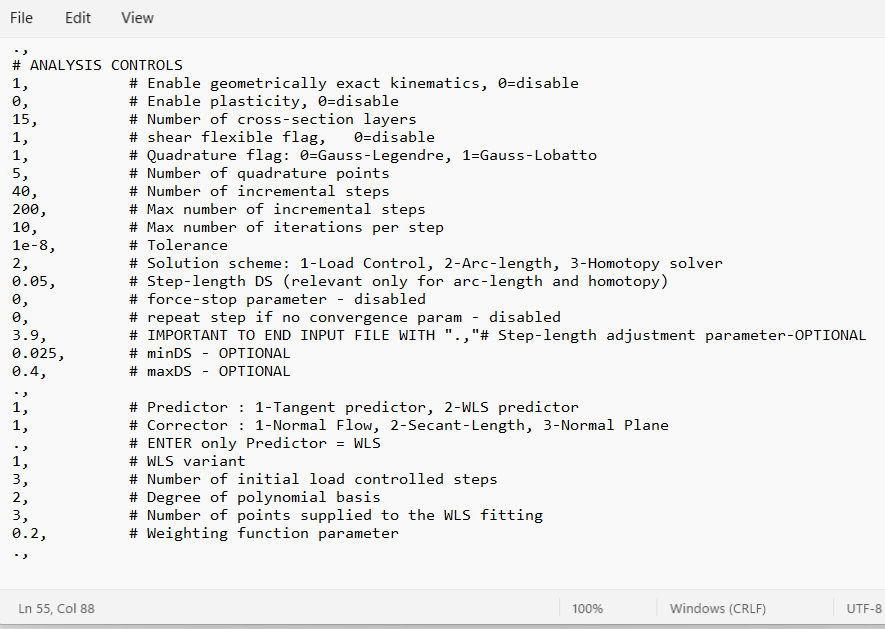
\includegraphics[scale=0.75]{GUIpics/INPUT_FILE/ANALYSISCONTROLS_TXT.png}
	\caption{The ANALYSIS CONTROLS template block for the ASCII input file.}
	\label{fig:ANALYSIS}
\end{figure}

\subsection*{The ANALYSIS CONTROLS input}
The final input block pertains to the \textit{Analysis Controls} tab in the 
\acrshort{gui}. 25 input parameters (rows) and only one column are required to 
fully 
specify and register the analysis settings. However, some of these options are 
read if the Homotopy solver is enabled. That leaves us with 18 ``core" 
parameters for this input block. The last three, which pertain to step-length 
adjustment parameter $a$ and minimum and maximum step-lengths, min$DS$ and 
max$DS$ respectively, are optional. If they are not specified, they are 
assigned the following default values:
\begin{itemize}
	\item $a=3.9$
	\item min$DS = DS/4$
	\item max$DS = 4DS$
\end{itemize}

\noindent where $DS$ is the standard step-length used by the arc-length and 
homotopy solvers. The template for this input block is shown in Fig. 
\ref{fig:ANALYSIS} below:

\subsection*{A Simple Problem Input File}

Here we show the input file and the U2-P2 equilibrium path on the application 
\acrshort{gui} for the elastoplastic cantilever problem analyzed in Chapter 
\ref{chapter:CH2}, Section \ref{CANTIPROB}.
\begin{figure}
	\centering
	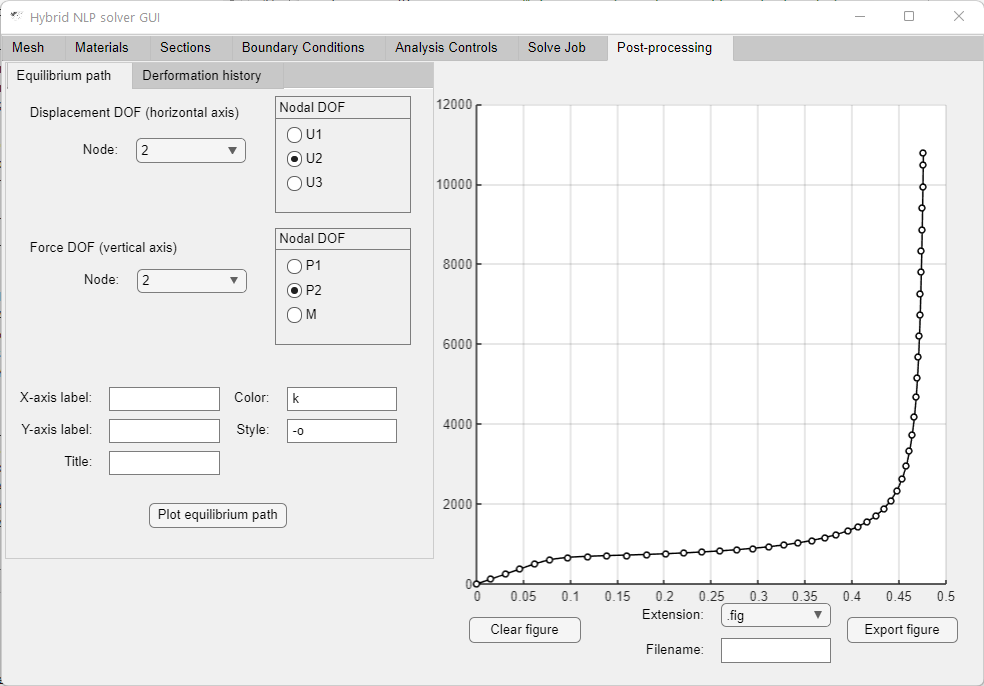
\includegraphics[scale=0.75]{GUIpics/INPUT_FILE/CANTIRES.png}
	\caption{The equilibrium plot for the elastoplastic cantilever, using the 
		GUI post-processor utility.}
	\label{fig:RES}
\end{figure}

\begin{figure}
	\centering
	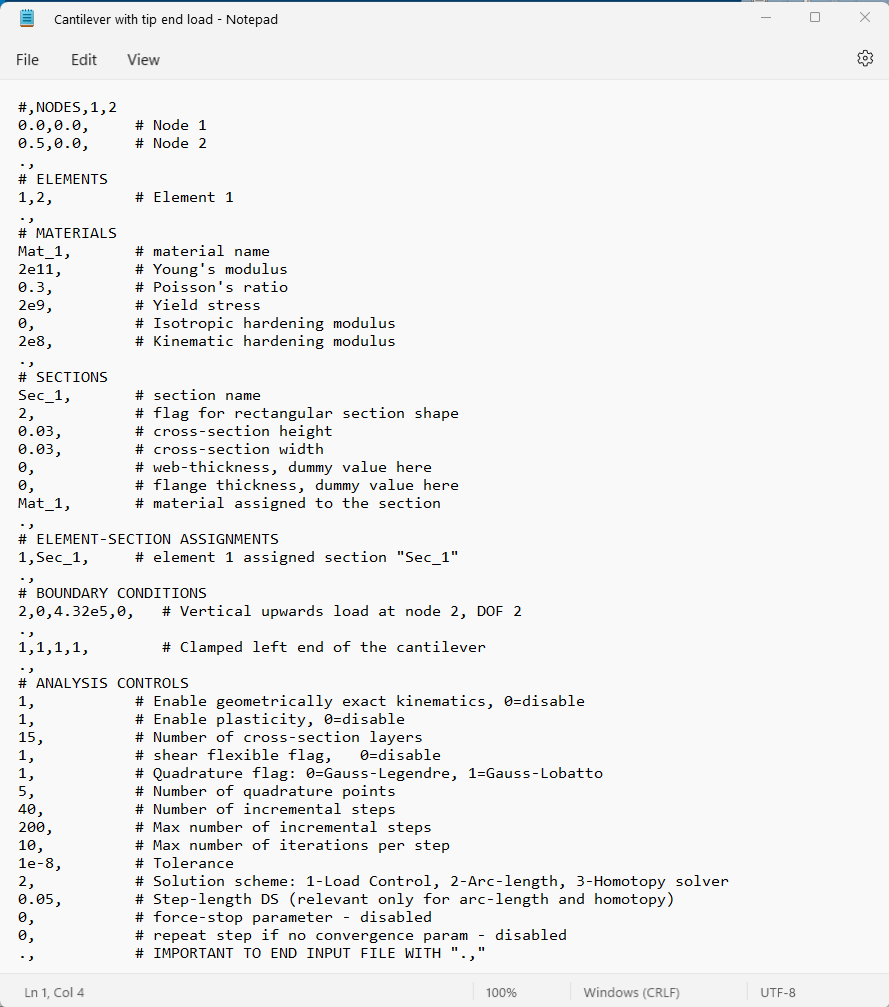
\includegraphics[scale=0.75]{GUIpics/INPUT_FILE/CANTI_TXT.png}
	\caption{The input file for a simple cantilever problem.}
	\label{fig:CANTINPUT}
\end{figure}

\subsection*{Input File for Matlab Source Code}

In this final section we will outline the basic structure of the input file 
when the user intends to use the source code directly. The source code is 
written in MATLAB and the problem input files are matlab functions. Figure 
\ref{fig:MAINFILE} below shows the core pre-processing and processing routines 
of the \textbf{main.m} file, which can be considered as the first and most 
primitive interface of the hybrid code.

Before the input file is read, the code ensures that the existing data in 
workspace memory are cleared and pertinent folders are added the search path. 
In addition, the directory \textit{output} is created if it does not exist 
already. If it does, all files inside that directory are deleted. This is the 
folder where we save the files where we write analysis output.

Then the problem input file is called (line 14 in \textbf{main.m}). The matlab 
function does not take any argument since everything is prepared by the user in 
the respective input file. However, in the case repeated parametric analyses 
are to be performed, the user will need to modify the function definition in 
the relevant input file so that it accepts pertinent arguments, if necessary. 
The input file function returns three Matlab \textbf{struct} data structures:

\begin{itemize}
	\item \textbf{snode}: Data structure where the coordinates, elements and 
	\acrshort{dof} status are stored for each node. Its dimension is equal to 
	the total number of nodes.
	\item \textbf{element}: Data structure where all parameters relevant to the 
	all elements are stored. Its dimension is equal to the total number of 
	elements.
	\item \textbf{anlsData}: Data structure where the general analysis settings 
	are stored. It contains 28 fields which will be briefly discussed below.
\end{itemize}

Next, the \textit{processInput.m} routine is called(line 18 in \textbf{main.m}) 
in order to perform the necessary pre-processing steps on the aforementioned 
data structures. Finally, the main processing routine, \textbf{solveJob.m}, is 
called once pre-processing is complete. It accepts the \textbf{anlsData} and 
\textbf{element} data structures, which it updates during the analysis and then 
returns them to be used by the post-processing routines.

\begin{figure}[t]
	\centering
	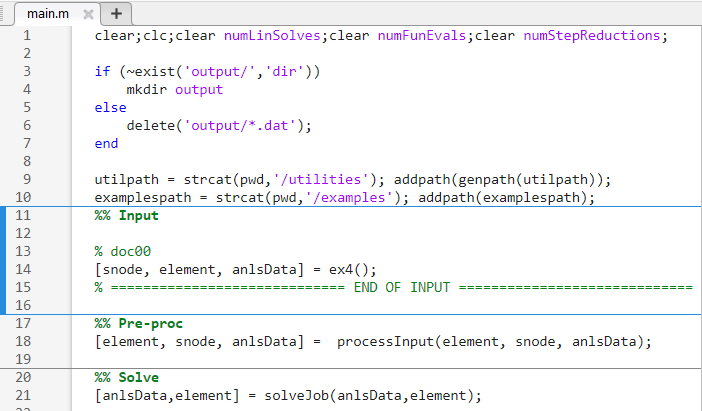
\includegraphics[scale=0.75]{FIG_MAINFILE.png}
	\caption{The \textbf{main.m} file of the hybrid code.}
	\label{fig:MAINFILE}
\end{figure}

When it comes to the input file layout, the user does not have to follow a 
strict sequence for parameter definition, however, it is highly recommended 
that a structured approach similar to the GUI input file is followed. In order 
to facilitate the exposition, a simple two-beam structure shown in Fig. 
\ref{fig:FIG_TOGGLEFRAME} will be used as input case. 

\begin{figure}
	\centering
	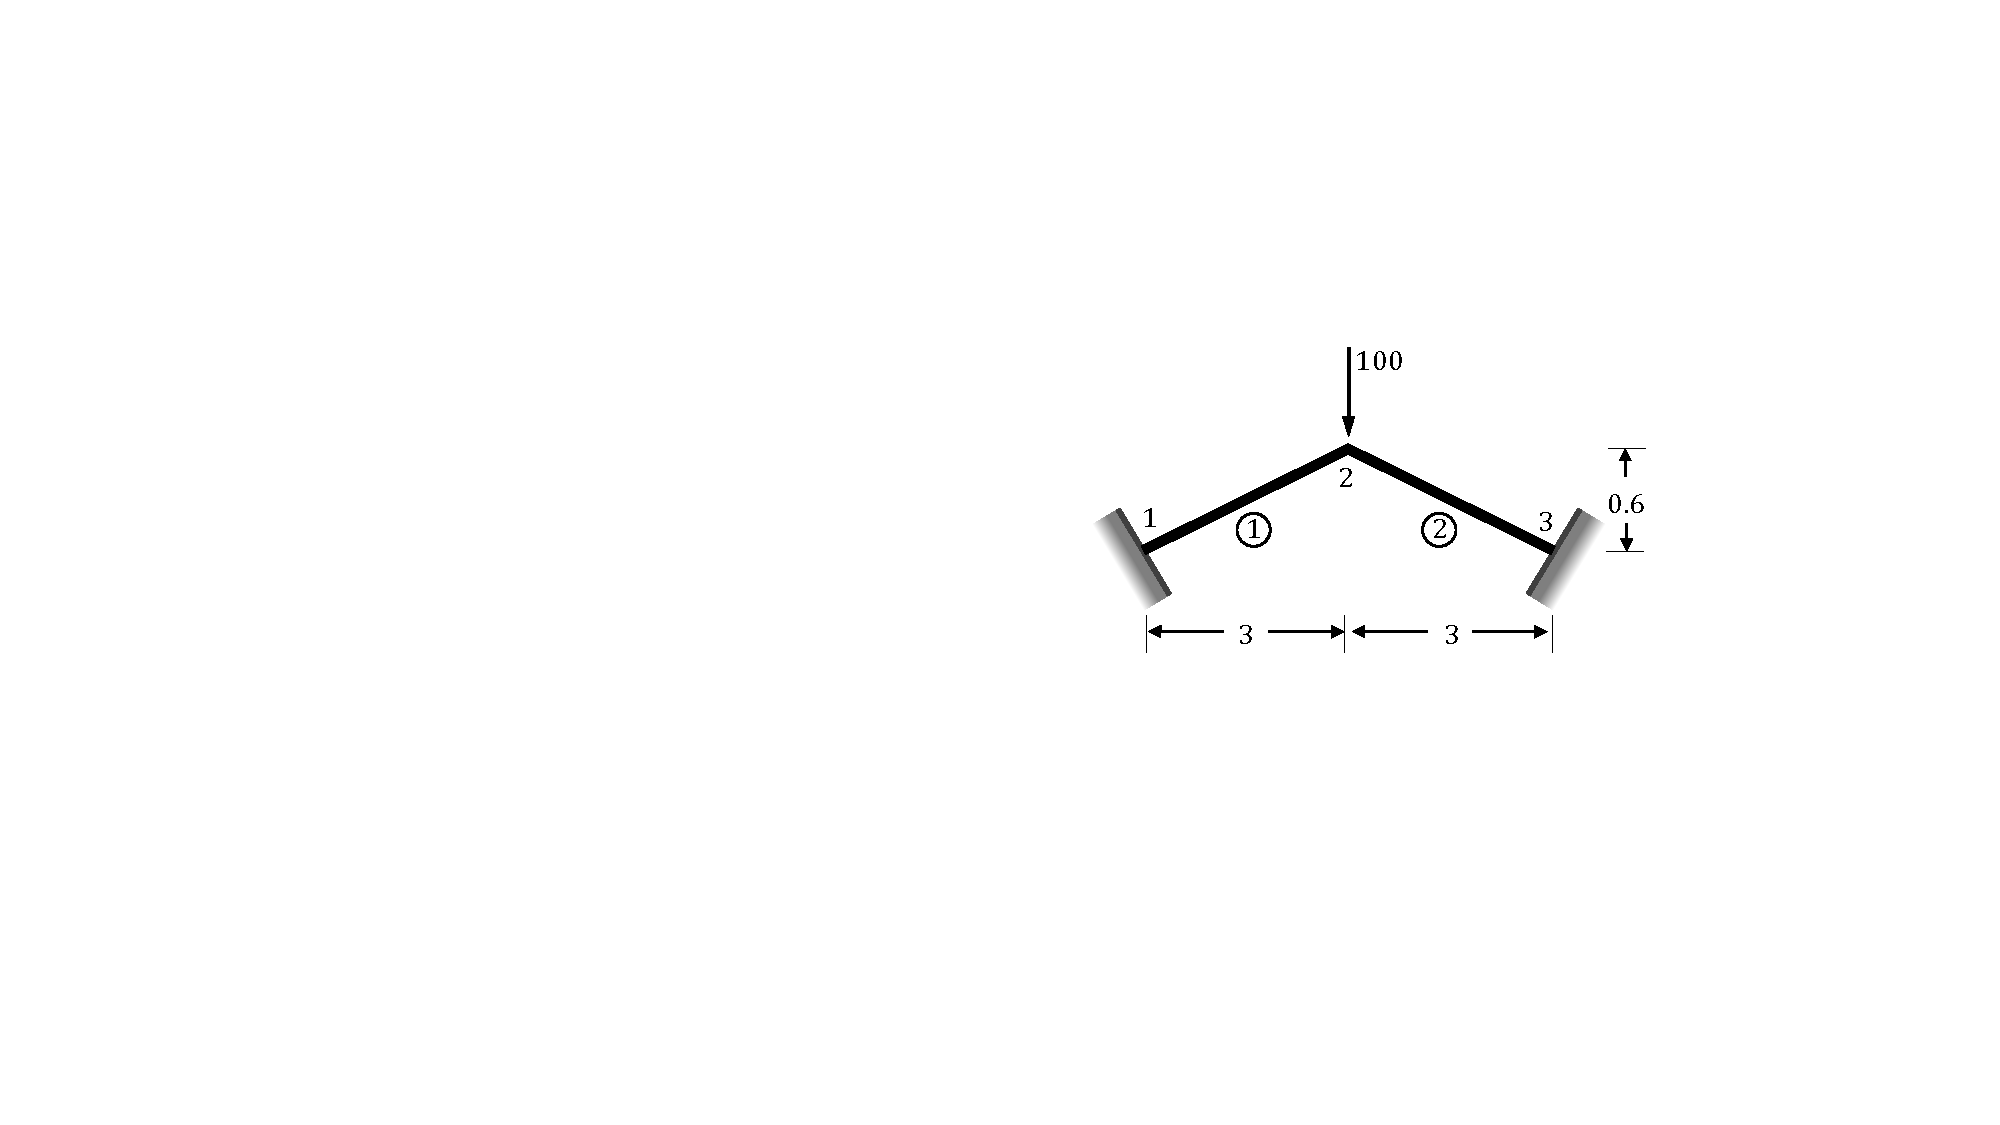
\includegraphics[scale=0.75]{FIG_TOGGLEFRAME}
	\caption{The geometry of the frame used as input.}
	\label{fig:FIG_TOGGLEFRAME}
\end{figure}

All sections in the matlab input file are shown in the figure sequence 
\ref{fig:FIG_INPUT1}, \ref{fig:FIG_INPUT2}, \ref{fig:FIG_INPUT3}, 
\ref{fig:FIG_INPUT4}.

\begin{figure}
	\centering
	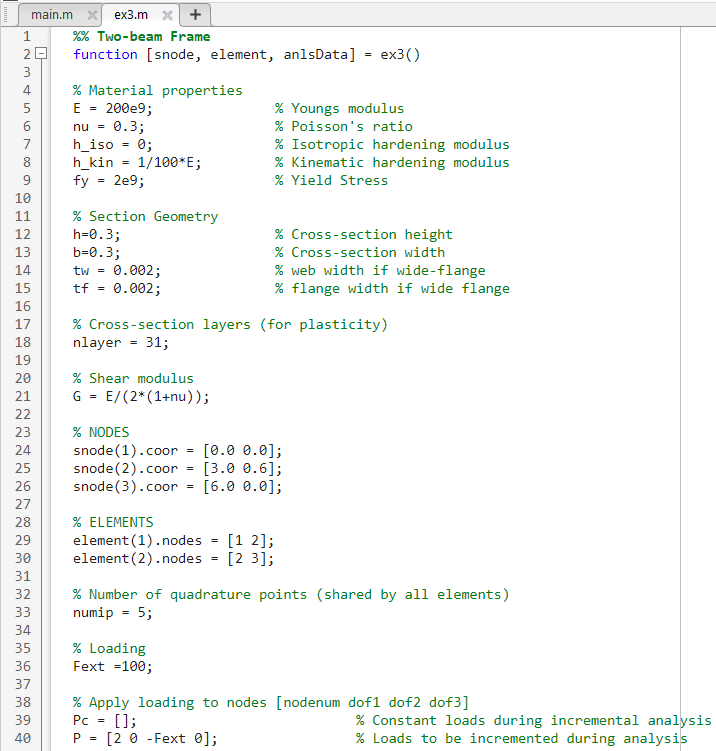
\includegraphics[scale=0.80]{FIG_INPUT1}
	\caption{First portion of Matlab input file.}
	\label{fig:FIG_INPUT1}
\end{figure}

\begin{figure}
	\centering
	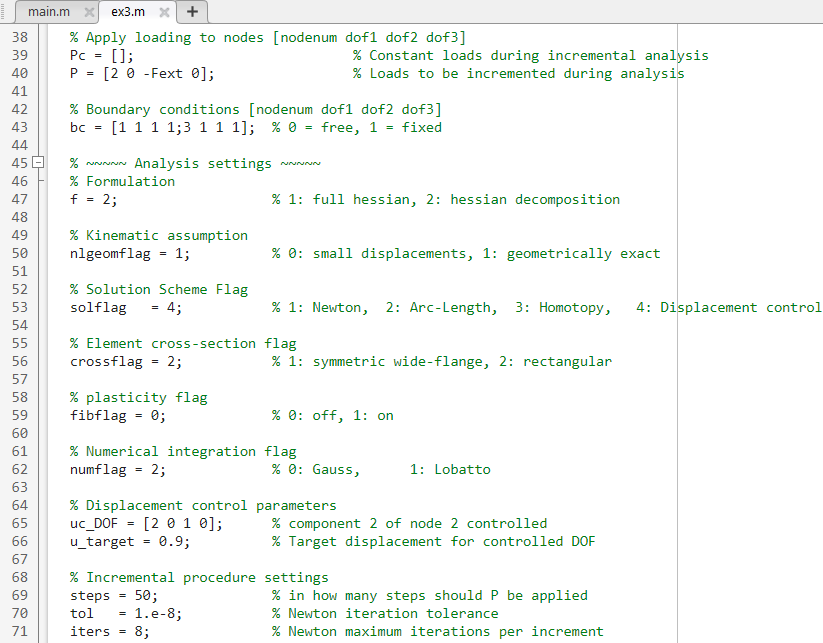
\includegraphics[scale=0.75]{FIG_INPUT2}
	\caption{Second portion of Matlab input file.}
	\label{fig:FIG_INPUT2}
\end{figure}

\begin{figure}
	\centering
	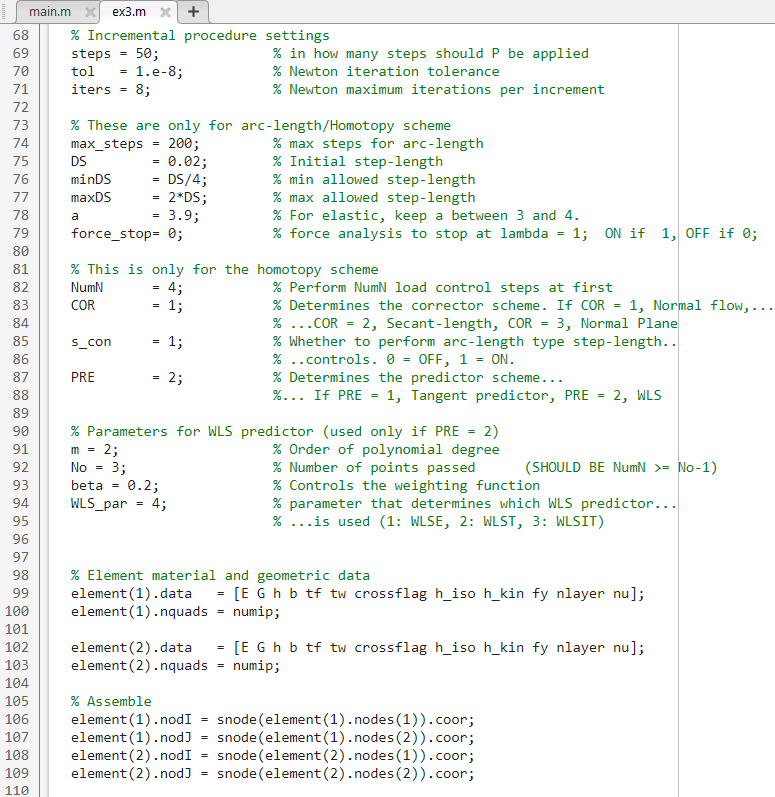
\includegraphics[scale=0.75]{FIG_INPUT3}
	\caption{Third portion of Matlab input file.}
	\label{fig:FIG_INPUT3}
\end{figure}

\begin{figure}
	\centering
	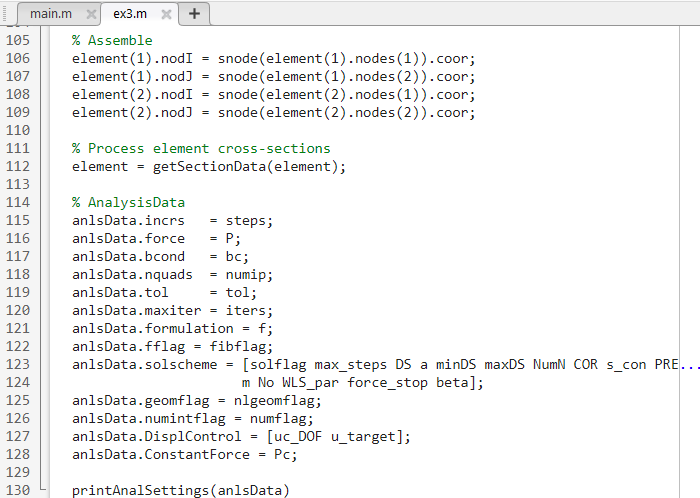
\includegraphics[scale=0.75]{FIG_INPUT4}
	\caption{Fourth and final portion of Matlab input file.}
	\label{fig:FIG_INPUT4}
\end{figure}

The parts pertinent to material and geometry definitions are similar in 
structure to the GUI input file. It is required that the user specifies a 
flange and web width even if a rectangular section is to be used. The values 
will be ignored in this case. The same holds for the fiber discretization. An 
integer value has to be assigned to variable \textit{nlayer} (line 18) even if 
an elastic analysis is scheduled. In that case, the value is, again, ignored.

As far as node and element definition, the user must assign the pertinent data 
directly to the corresponding structure. For the definition of 
node $n$, a $1\times 2$ vector containing the $x$ and $y$ coordinates is 
assigned directly to field \textit{coor} of the $n$-th component of structure 
\textbf{snode} as follows:
\begin{center}
	\textbf{snode(n).coor} = [1.25 0.5];
\end{center}

\noindent See also lines 24-26 in Fig. \ref{fig:FIG_INPUT1}. In a similar 
fashion, for the definition of element $m$, we assign the vector $[node_I\  
node_J]$ directly to field \textit{nodes} of the $m$-th component of structure 
\textbf{element}, as shown in lines 29-30 of Fig. \ref{fig:FIG_INPUT1}. The 
general format is:

\begin{center}
	\textbf{element(m).nodes} = [2 3];
\end{center}
\noindent where element $m$ connects $node_I=2$ and $node_J=3$.

For each parameter that needs to be defined by the user there are brief but 
detailed tooltips in the form of comments on the same line. Two features that 
are available in this form of input but are not in the GUI version are 1) the 
option to define ``gravity'' loads which remain constant throughout the 
analysis and 2) the option to perform a displacement control incremental 
analysis. If this option is chosen (see line 53 in Fig. \ref{fig:FIG_INPUT2}), 
then the user needs to also specify the nodal \acrshort{dof} that is controlled 
and the target displacement up to which the said \acrshort{dof} is to be 
incremented to. The relevant lines for these definitions are 65-66 in Fig. 
\ref{fig:FIG_INPUT2}.

The user can choose any name for the variables they define, however they should 
ensure that all variables are stored in a consistent fashion and the 
correspondence with the basic data structures \textbf{snode}, \textbf{element} 
and \textbf{anlsData} is not spoiled. As can be seen in the third and fourth 
portions of the input file in Figs. \ref{fig:FIG_INPUT3}, \ref{fig:FIG_INPUT4}, 
if a different name is chosen for a parameter (left-hand side during 
definition), then the same name has to be assigned to the relevant structure 
field (right-hand side during assignment). In addition, using Matlab functions 
to do analysis with the hybrid code, while more versatile, it is also more 
error-prone. The numerous error checks implemented for the \acrshort{gui} 
version are not carried out when setting up a problem using Matlab input files, 
so users should be more cautious in the latter case.

\subsubsection*{The main data structures}

As mentioned earlier, the three main data structures are 1) \textbf{snode}, 2) 
\textbf{element} and 3) \textbf{anlsData}. For the structure in Fig. 
\ref{fig:FIG_TOGGLEFRAME}, the \textbf{snode} data structure with its fields 
are shown Fig. \ref{fig:FIG_SNODE}. For a particular node m, \textbf{snode(m)}, 
the \textit{els} field is a vector with components the labels (integers) of 
those elements that include node m. The field \textit{dofstatus} returns a 
vector that contains the nodal \acrshort{dof}s for node m that are restrained. 
For example, since node 1 in the frame above is fixed on the ground, then the 
field returns \textbf{snode(1).dofstatus} = [1 2 3] since all 3 \acrshort{dof}s 
are restrained. If no \acrshort{dof}s are restrained, \textit{dofstatus} 
returns an empty vector. 



\begin{figure}
	\centering
	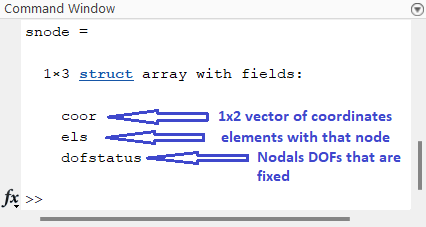
\includegraphics[scale=0.90]{FIG_SNODE}
	\caption{The \textbf{snode} data structure.}
	\label{fig:FIG_SNODE}
\end{figure}

Next, we have the \textbf{element} structure, which is used to store data 
pertaining to individual elements that will be used and updated during analysis 
and, then, stored for post-processing purposes. The relevant fields are shown 
in Fig. \ref{fig:FIG_element_struct} for the 2-beam frame. We can see that 
\textbf{element} is of 
dimension 2, since there are only two elements. For most fields, the 
description added in the figure is adequate. The field \textit{data} is a 
$1\times 11$ vector that contains the following parameters:

\begin{center}
	\textbf{element(m).data} = $[E\ G\ A\ I\ H_{iso}\ H_{kin}\ n_l\ k_s\ u_p]$
\end{center}
	
	\noindent where these parameters are: Young's modulus, shear modulus, 
	cross-section area, moment of inertia, isotropic hardening modulus, 
	kinematic 
	hardening modulus, $n_l$ is the number of layers, shear coefficient and, 
	lastly, $u_p$ is a 
	parameter given by the following integral over a cross-section:
	
	$$ u_p = \int_A \varphi(X_2)^2\text{d}A $$
	
	\noindent and is used to determine the shear coefficient $k_q$ for 
	quadratic 
	shear strain distribution (see Eqs. \ref{eq:SHEAR_COEFF}, 
	\ref{eq:QUAD_COEFF}). The \textit{secArrays} field returns a $2\times n_l$ 
	vector where the first column contains the area of fibers and the second 
	contains the heights of these fibers on the cross-section. The field 
	\textit{gradHyb} stores matrix $\nabla_{\mathbf{y}_i}\bvec{h}_g^B$, given 
	in Appendix \ref{eq:grad_Hb_y}, at each element quadrature point. 
	
	\begin{figure}
		\centering
		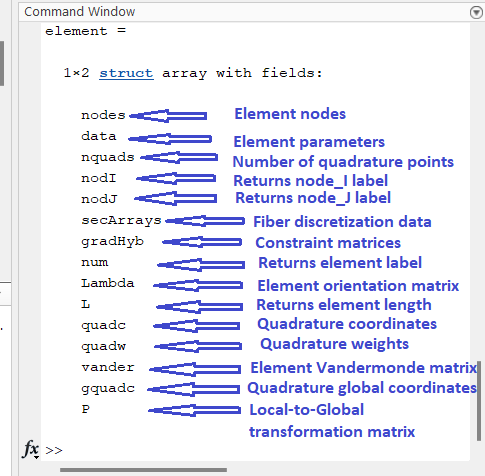
\includegraphics[scale=0.85]{FIG_element_struct}
		\caption{The \textbf{element} data structure.}
		\label{fig:FIG_element_struct}
	\end{figure}


Lastly, we use the \textbf{anlsData} structure to store all parameters 
pertaining to the analysis settings. Its dimension is one and the relevant 
fields it encapsulates are shown in Fig. \ref{fig:FIG_anlsData}. Again, short 
descriptions are 
provided in the figure and below we discuss certain fields whose use might not 
be apparent. 

The \textit{incrs} field returns the number of incremental steps for the 
Load-Controlled Newton method. It is overridden by parameter max\_steps (see 
Line 74 in Fig. \ref{fig:FIG_INPUT3}), which is stored in the second place of 
field \textit{solscheme}. Both \textit{force} and \textit{bcond} fields, which 
pertain to external loading and support specification respectively, are defined 
to in the 
same way as with the \acrshort{gui} input. Field \textit{formulation} 
determines which solver is 
called to handle the linearized system of the Lagrangian gradient. It should 
always be set to 2, which leads to a solution by block elimination of the 
Hessian. The \textit{ConstantForce} field returns the vector of ``gravity'' 
loads that remain constant during the incremental analysis. While the proper 
way to handle the presence of such loads is to perform a separate initial, 
usually load-controlled analysis and then proceed with the nonlinear 
incremental analysis by using the solution of the former one as starting state, 
presently, no such approach is followed. Instead, all loads are assumed to be 
present from the start and only the loads in the \textit{force} field are 
incremented. For that reason, caution is advised when setting values for the 
gravity loads, since large values might cause early termination due to the 
solution not being close to the initial state. The \textit{Hessian} and 
\textit{Gradient} fields return the updated Hessian and Gradient of the 
Lagrangian, respectively, for the whole structure for the current step. When 
the analysis is concluded, both of these objects pertain to the last step. The 
field \textit{totdofs} returns the total number of \acrshort{dof}s for the 
problem, including Lagrange multipliers. The \textit{dhis} stores nodal 
displacements and quadrature point strain measures for each step, which are 
then used for post-processing purposes. Field $\lambda$ is the homotopy 
parameter. When the load is parameterized in the context of the 
\acrshort{npnlp} framework, this field returns a vector with the values of the 
load proportionality parameter at each step. The field \textit{CurveLength} 
stores the length of the homotopy/equilibrium curve up to each step. It returns 
a $1\times steps$ vector. Field \textit{ResultantHis} stores the three 
stress resultants at all nodes and all element quadrature points at each step. 
If Displacement Control is selected, then the additional necessary data are 
stored in the \textit{DisplControl}. The \textit{numintflag} field determines 
the quadrature rule. If \textit{numintflag=1} then the Gauss-Lobatto quadrature 
will be used, while for Gauss-Legendre, the option is again set 
to\textit{numintflag=0}. 
Lastly, the \textit{solscheme} field stores the following analysis parameters:
\begin{center}
	\textbf{anlsData.solscheme} = [solflag max\_steps $\Delta S$ 
	min$\Delta S$ max$\Delta S$ NumN COR s\_con PRE m N\_o 
	WLS\_par force\_stop beta]
\end{center}

\noindent
\begin{itemize}
	\item \textbf{solflag} is the flag that determines which solver is used 
	(see Line 
	53, Fig. \ref{fig:FIG_INPUT2}).
	\item \textbf{max\_steps} determines the maximum number of incremental 
	steps.
	\item $\Delta S$ is the step-length when the arc-length or the homotopy 
	solvers are used.
	\item min$\Delta S$ is the minimum allowed step-length. 
	\item max$\Delta S$ is the maximum allowed step-length. 
	\item \textbf{NumN} is the number of load-controlled steps to perform 
	before 
	switching to \acrshort{wls} predictor.
	\item \textbf{COR} specifies which corrector is to be used. If 
	\textbf{COR=1}, the Normal 
	Flow corrector is used. If \textbf{COR=2}, the arc-length/secant-length 
	correctors 
	are used. if \textbf{COR=3}, the Normal Plane corrector is used.
	\item \textbf{s\_con} determines whether step-length controls are to be 
	performed. If \textbf{s\_con =1}, then $\Delta S$ is adjusted at the end of 
	each 
	step.
	\item \textbf{PRE} determines which predictor will be used. If 
	\textbf{PRE=1} then the 
	tangent predictor is used. If \textbf{PRE=2} then the \acrshort{wls} 
	predictor is 
	used.
	\item \textbf{m} determines the order of polynomial basis for the 
	\acrshort{wls} 
	approximation.
	\item \textbf{N\_o} specifies the number of previously converged points 
	passed to 
	the \acrshort{wls} predictor.
	\item \textbf{WLS\_par} determines which \acrshort{wls} predictor variant 
	is to 
	be used. For \textbf{WLS\_par}=1, then the predictor is \acrshort{wlse}, 
	while 
	for \textbf{WLS\_par=2} and \textbf{WLS\_par=3}, the predictors are the 
	\acrshort{wlst} and \acrshort{wlsit} respectively.
	\item \textbf{force\_stop} is a flag that determines if analysis should 
	stop when 
	the load proportionality parameter becomes larger than 1.
	\item \textbf{beta} is the weighting function parameter used in the 
	\acrshort{wls} 
	predictor. 
\end{itemize}

	\begin{figure}
		\centering
		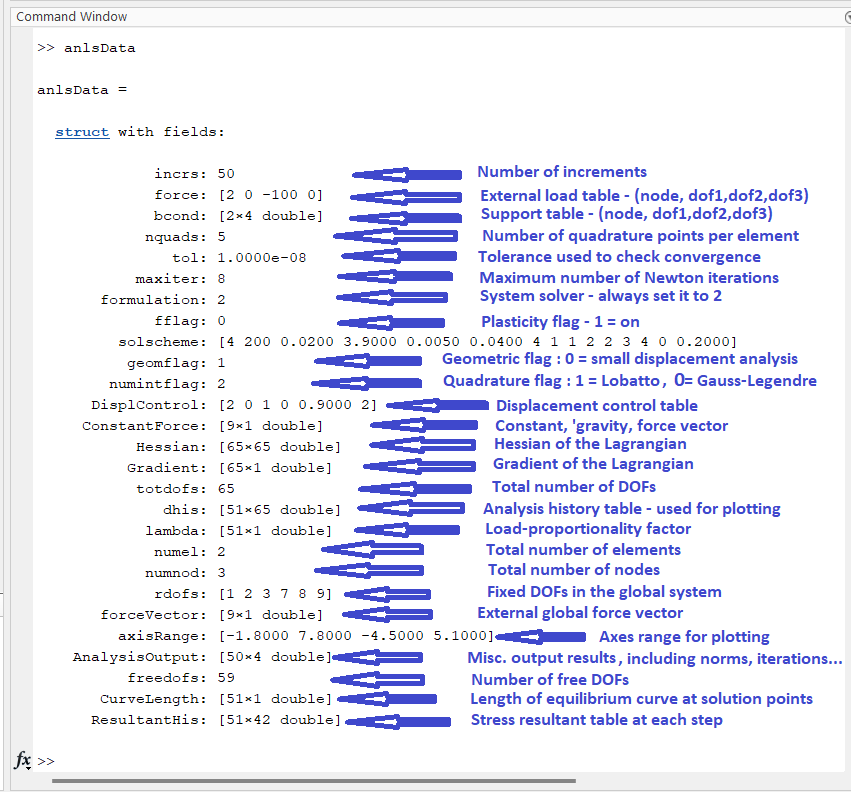
\includegraphics[scale=0.85]{FIG_anlsData}
		\caption{The \textbf{anlsData} data structure.}
		\label{fig:FIG_anlsData}
	\end{figure}
\end{appendices}